%------------------------------------------------------------------------------
\def\todaysdate{20190108}
\newday{\todaysdate}\label{\todaysdate}

\newentry[Racking]{1900 Racking}
\FloatBarrier{}

\begin{my_itemize}
    \item Assembled the new transfer pump.  I cut the supplied hose in half, and attached one side of each half to the pump, then the source side to the stainless steel racking cane, and the other side to a beer side ball lock connector.
    \item A gas side ball lock disconnect with no fittings was attached to the other post to allow air to vent.
    \item I attached the ball lock to the target cornelius keg, and inserted the racking cane into a gallon milk jug filled with sanitizer.  I pumped several cups of water into the cornelius keg, and then shook the cornelius keg making sure the sanitizer was splashed against all sides of the keg.  I let the solution sit for two minutes, then opened the keg and poured out the sanitizer, and pumped out the remaining sanitizer in the lines.  I then opened the primary fermentation bucket inserted the racking cane about an inch below the surface, and started the pump.  As I neared the bottom I tilted the bucket to get the last bit.
    \item The beer has a nice dark color, and there was sign of a good amount of krausen on the sides of the bucket but not on the beer.  The layer of trub was about 1/2 inch thick.
    \item The content of the bucket was slightly more than the capacity of the keg, and a bit sprayed out of the vent at the end across my basement.  A future improvement could be to add a hose to the air vent and drop it into a bucket in case of overflows.
\end{my_itemize}

\begin{figure}[H]
  \centering
  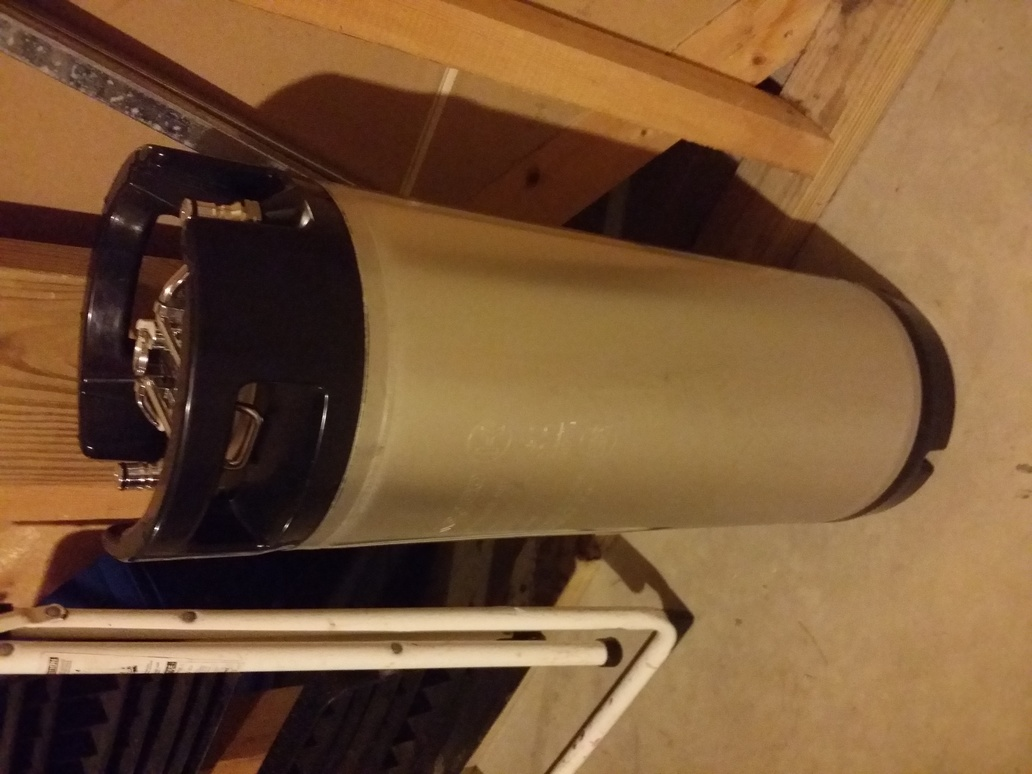
\includegraphics[angle=270,origin=c,width=0.5\textwidth]{IMG_20190108_195458_reduced}
  \caption{Force Carbonation}\label{fig:racking:complete}
\end{figure}

\begin{figure}[H]
  \centering
  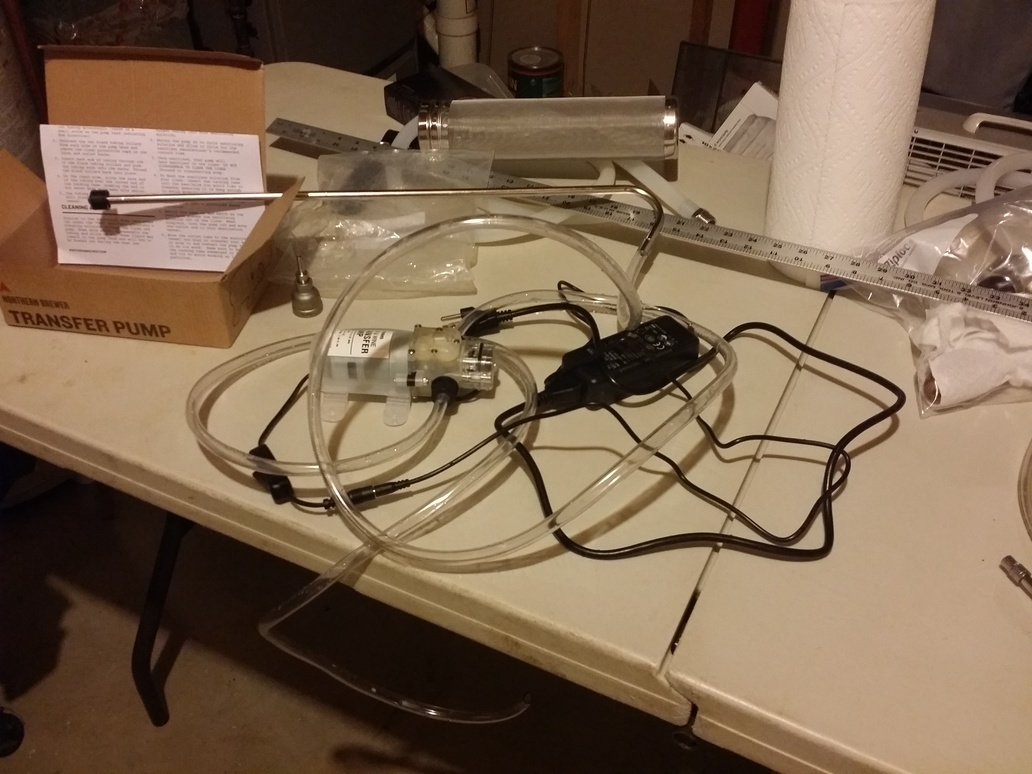
\includegraphics[angle=0,origin=c,width=\textwidth]{IMG_20190108_195511_reduced}
  \caption{Force Carbonation}\label{fig:racking:transferpump}
\end{figure}

\FloatBarrier{}
\clearpage
%------------------------------------------------------------------------------
\def\todaysdate{20190111}
\newday{\todaysdate}\label{\todaysdate}

\newentry[Beginning Force Carbonation]{1900 Beginning Force Carbonation}
\FloatBarrier{}

\begin{my_itemize}
    \item Assembled the force carbonization hardware.
    \item I swapped out the regulator on my kegerator for the new one I bought for force carbonating.  The one on my kegerator was very difficult to keep dialied into a setting.  The new regulator seems to be of a much higher quality.  I will put the better regulator on the serving system, the kegerator, and use the lesser regulator to force carbonate.
    \item A CO2 hose was attached to the regulator's hose barb, which was a 5/16'' barb, and to the barb on the gas ball lock disconnect.  The barb on the gas ball lock was only a 1/4'', so I wrapped several layers of silicone tape over the barb before inserting it into the hose.  I also used two clamps on this side of the hose.  This provided an airtight seal.
    \item The ball lock was attached to the corny keg, and the pressure release valve was pulled several times to make sure the air was purged from the keg and that only CO2 remained.  The pressure on the CO2 regulator was left at 10psi.
\end{my_itemize}

\begin{figure}[H]
  \centering
  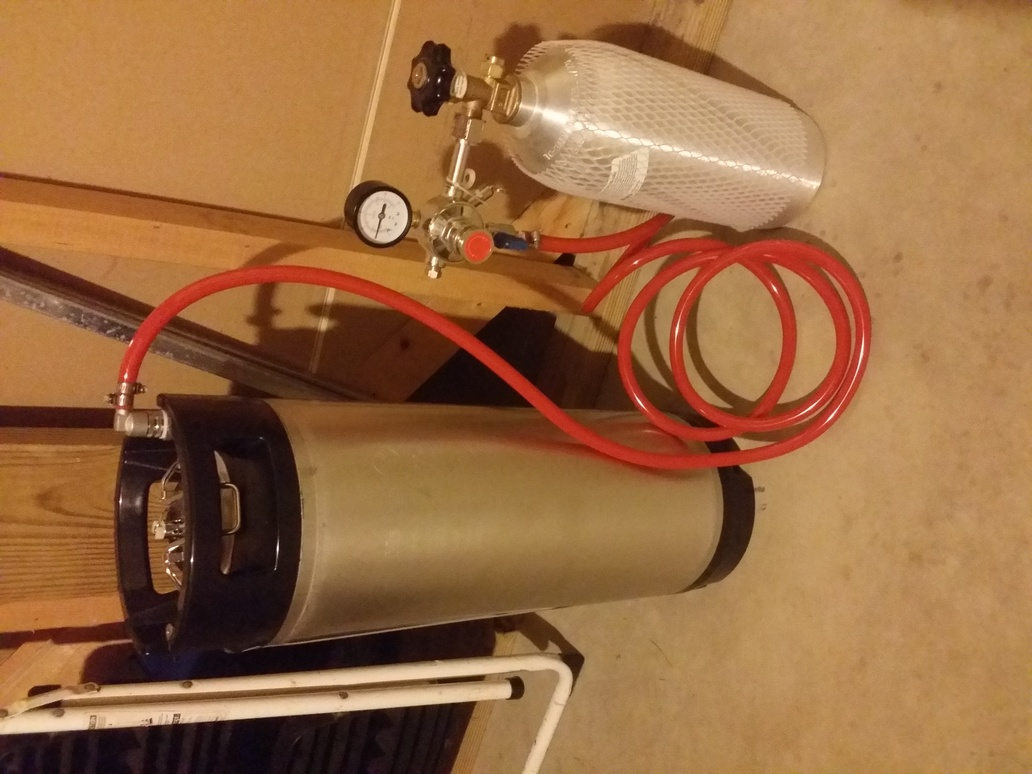
\includegraphics[angle=270,origin=c,width=0.5\textwidth]{IMG_20190111_212159_reduced}
  \caption{Force Carbonation}\label{fig:forcecarbonation}
\end{figure}

\FloatBarrier{}
\clearpage

%------------------------------------------------------------------------------
\def\todaysdate{20190111}
\newday{\todaysdate}\label{\todaysdate}

\newentry[Sample]{1900 Sample}
\FloatBarrier{}

A faucet was installed on the beer post with a quick connect adapter.  The faucet is a perlick.  For future reference, perlicks are wonderful faucets, but there is no spring loaded close off of the valve.  When I attached the faucet, the keg was under pressure, and the valve was open.  So another spill occurred in the basement, shown in figure~\ref{fig:sample:mishap}.  After a few minutes of cleaning up concrete, I was able to draw a sample.

Figures~\ref{fig:sample:1} and~\ref{fig:sample:2} show the sample that was drawn.  Tasting shows no ``off'' flavors.  That is, no hints of milk, apple, cardboard, or anything else other than a subtly hopped dark but a bit flat beer.

The faucet was removed from the keg, and the CO\textsubscript{2}, and the keg was installed in the kegerator upstairs to just the CO\textsubscript{2} line.  I want to clean the beer lines before connecting to this new keg as the kegerator has been empty, but refridgerated for over a month.  The temperature was dialed in at 42 degrees, and the pressure set for 20psi.  After two days at this temperature and pressure, I plan to dial the pressure down to 10psi.

Funny Story:  My kids got a google mini for Christmas, and when they are board, have been playing with the new features.  It just happens they had it sitting on top of my kegerator because there was a power outlet near by, and it just happened that the kids were playing with their tablet in the other room just as I finished installing the keg.  So right after I install the keg, and close the door to the kegerator, the kegerator says to me ``I love you daddy!''.  They had just discovered the ``broadcast a voice message'' feature.

\begin{figure}[H]
  \centering
  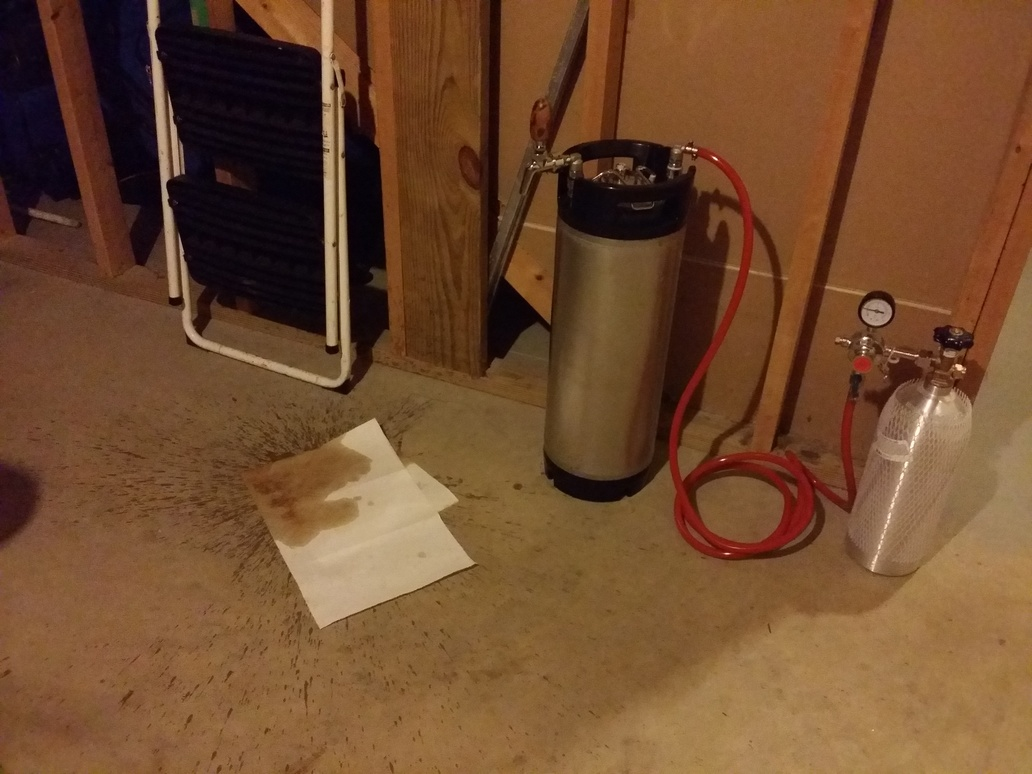
\includegraphics[angle=0,origin=c,width=\textwidth]{IMG_20190114_182953_reduced}
  \caption{Sample mishap}\label{fig:sample:mishap}
\end{figure}

\begin{figure}[H]
\begin{minipage}{0.45\textwidth}
  \centering
  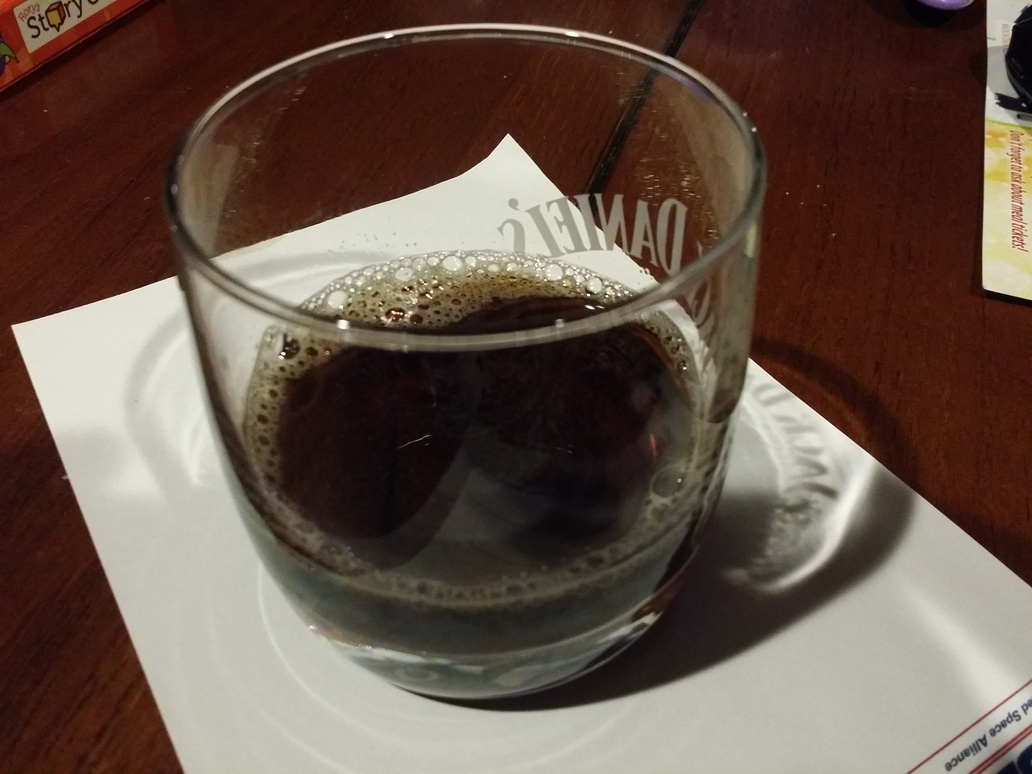
\includegraphics[width=\textwidth]{IMG_20190114_183506_reduced}
  \caption{Sample View 1}\label{fig:sample:1}
\end{minipage}\hfill
\begin{minipage}{0.45\textwidth}
  \centering
  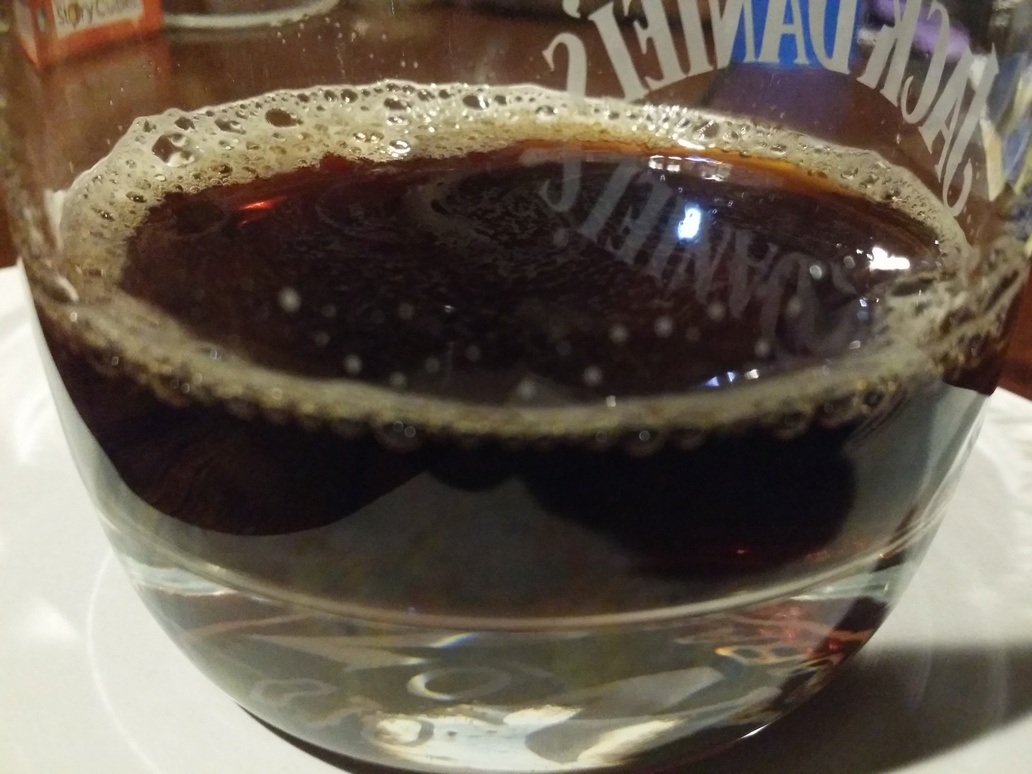
\includegraphics[width=\textwidth]{IMG_20190114_183526_reduced}
  \caption{Sample View 2}\label{fig:sample:2}
\end{minipage}
\end{figure}

\FloatBarrier{}
\clearpage

\begin{figure}[H]
  \centering
  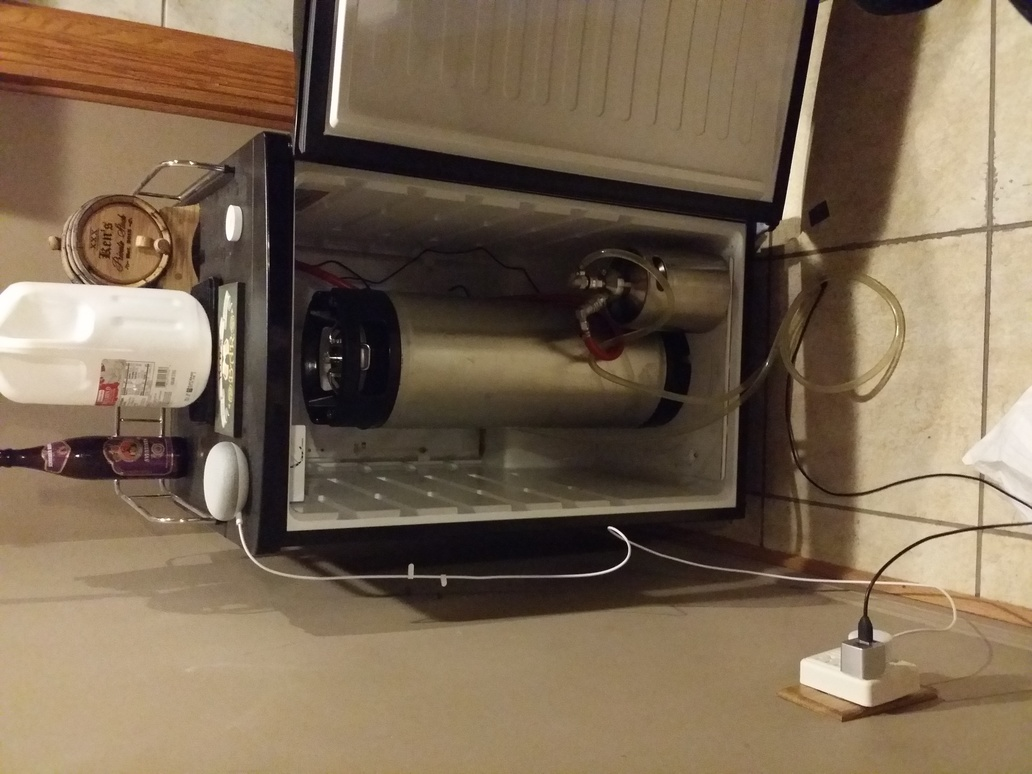
\includegraphics[angle=270,origin=c,width=0.5\textwidth]{IMG_20190115_204926_reduced}
  \caption{Cleaning kegerator lines}\label{fig:cleaning}
\end{figure}

\begin{figure}[H]
  \centering
  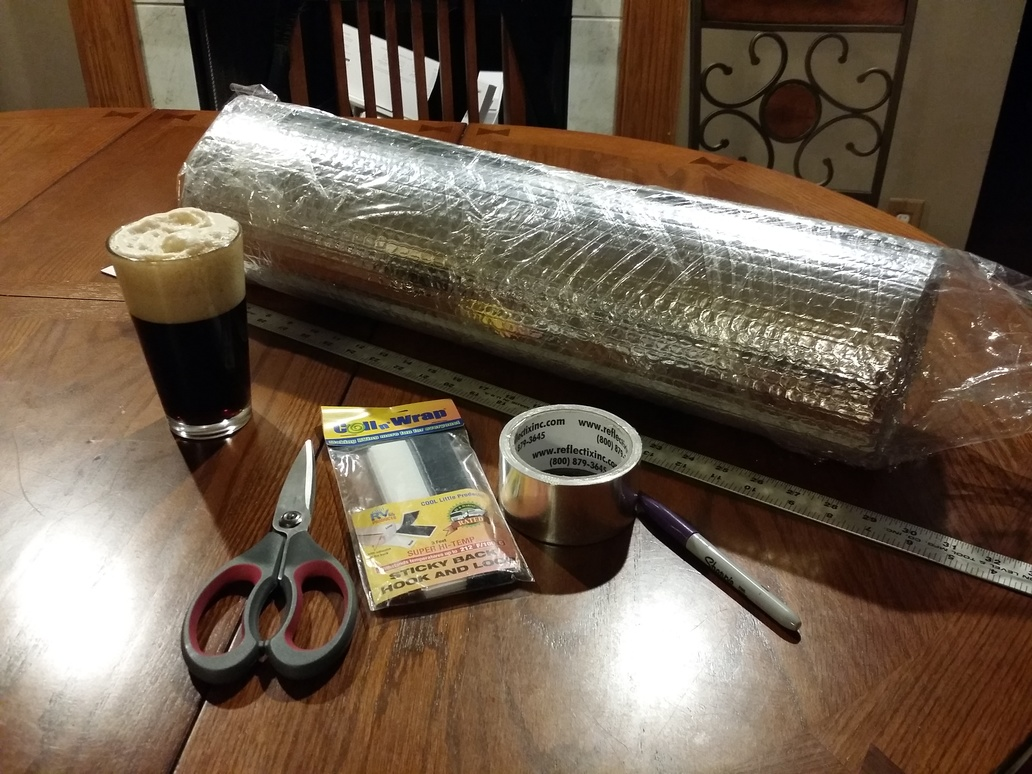
\includegraphics[width=\textwidth]{IMG_20190119_172654_reduced}
  \caption{Preparing to make brew jacket}\label{fig:brewjacket:prep}
\end{figure}

\begin{figure}[H]
  \centering
  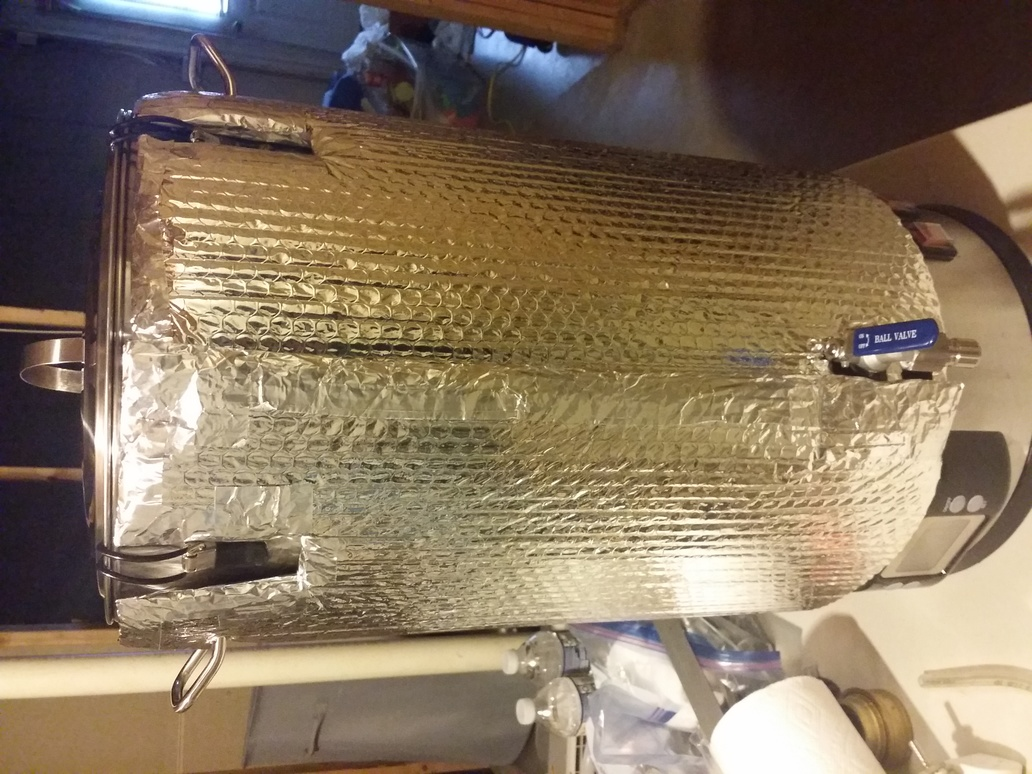
\includegraphics[angle=270,origin=c,width=0.5\textwidth]{IMG_20190120_121041_reduced}
  \caption{Completed Brew Jacket Side View}\label{fig:brewjacket:side}
\end{figure}

\begin{figure}[H]
  \centering
  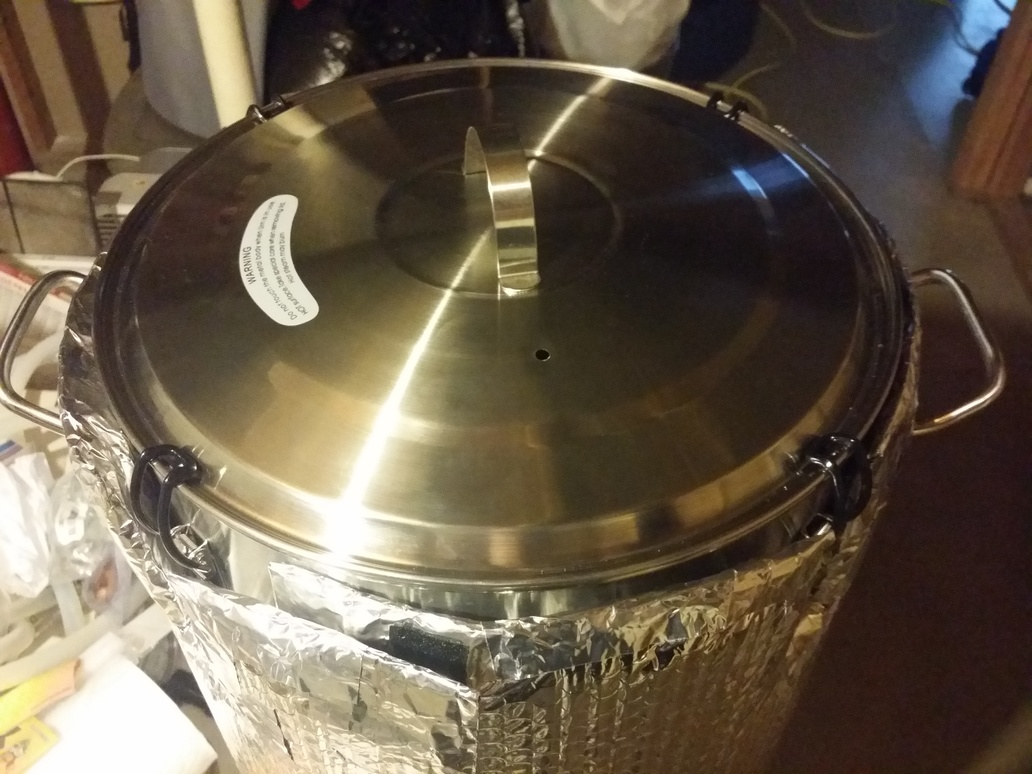
\includegraphics[width=\textwidth]{IMG_20190120_121055_reduced}
  \caption{Completed Brew Jacket Top View}\label{fig:brewjacket:top}
\end{figure}

\begin{figure}[H]
  \centering
  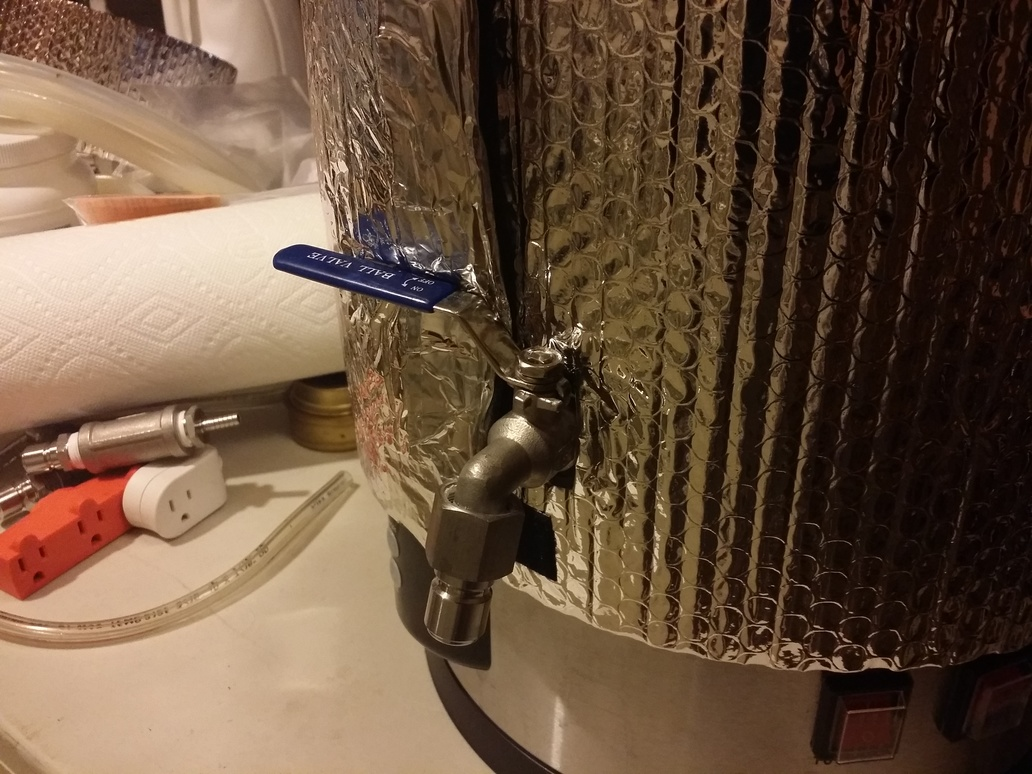
\includegraphics[width=\textwidth]{IMG_20190120_121114_reduced}
  \caption{Completed Brew Jacket Valve Closeup}\label{fig:brewjacket:valve}
\end{figure}

%------------------------------------------------------------------------------
\def\todaysdate{20190126}
\newday{\todaysdate}\label{\todaysdate}

\newentry[Brew]{0754 Brew}
\FloatBarrier{}
1721 Mixed up a gallon of sanitizer.  One step, 1 tbsp.

1725 Added 4.5 gallons to mash tun as read by the markers on the inside of the mash tun, set to heat to 173

1736 Placed air trap and yeast in sanitizer in bowl, set aside

1742 Sanitized a small piece of beer tube.  Will place this between filter and stone in aerator.

1744 Sprayed everclear into aeration stone

1803 Added Added just short of to the 13 L mark water to the sparge water heater, and turned on the heat

1807 Drank a beer from the last batch

1823 Mash Tun water temp reached 173, Beginning Mash in

1833 Mash in complete, temp is 164, leaving lid off of top to allow heat to escape

1837 Temp is down to 162

1845 Temp is down to 158

1856 Temp is down to 154 Placed lid back on mash tun

1904 Temp is 152

1921 Temp is 148 (Note Warmer kicks in at 6 degrees below set temperature)

1933 Lifted basket, started recirculating wort, set heater to 165

1943 Shut off pump and closed valve on mash tun, started pump, and opened valve on sparge water heater, watching for 10.4 L of water to transfer  Note the white line between 75 and 80 on the sparge water heater seems to correspond to the correct sparge water temperature.

2019 10.4 L of water completed transfer to top.  I tried to maintain about one inch of water over the grain bed, it was pretty easy to dial in the speed to do that, ask damon later if the full hour should be spent transferring sparge water or if it is ok to sparge for 30 minutes, then drain for 30 minutes.  Note, there is still a slow leak on the sparge water faucet, it is coming out between the quick connect and the spicot

2034 Leak started to get worse.  Used some X-TREME tape on the connection, and the leak has stopped.

2043 Set heater to 220.  Note: Since it takes a while to get to boil, I should have started the heater at 30 minutes into sparge, the sparging basket could have completed draining while the water was coming up to temperature.

2050 Removed sparging basket.  Wort level is at 6 Gallon mark on mash tun

2113 214 degrees reached according to mash tun, 1 hour timer started, adding challenger hops in hop spider.  While opening the hops, the kettle almost boiled over.  The hop spyder when placed in cut down the foam almost instantly.

2145 Drinking Beer

-15 Added irish moss

-5 Added willamette and turned on pump, temperature dropped to 203 and boil has stopped

2230 Yeast pitched, stirred, tilt was added after sitting in sanitizer for 10 minutes, and the airlock was installed and filled.  Ended up with about 5.15 gallons of wort, with 1.050 OG

01/27/2019
0101 Done Cleaning

\begin{figure}[H]
  \centering
  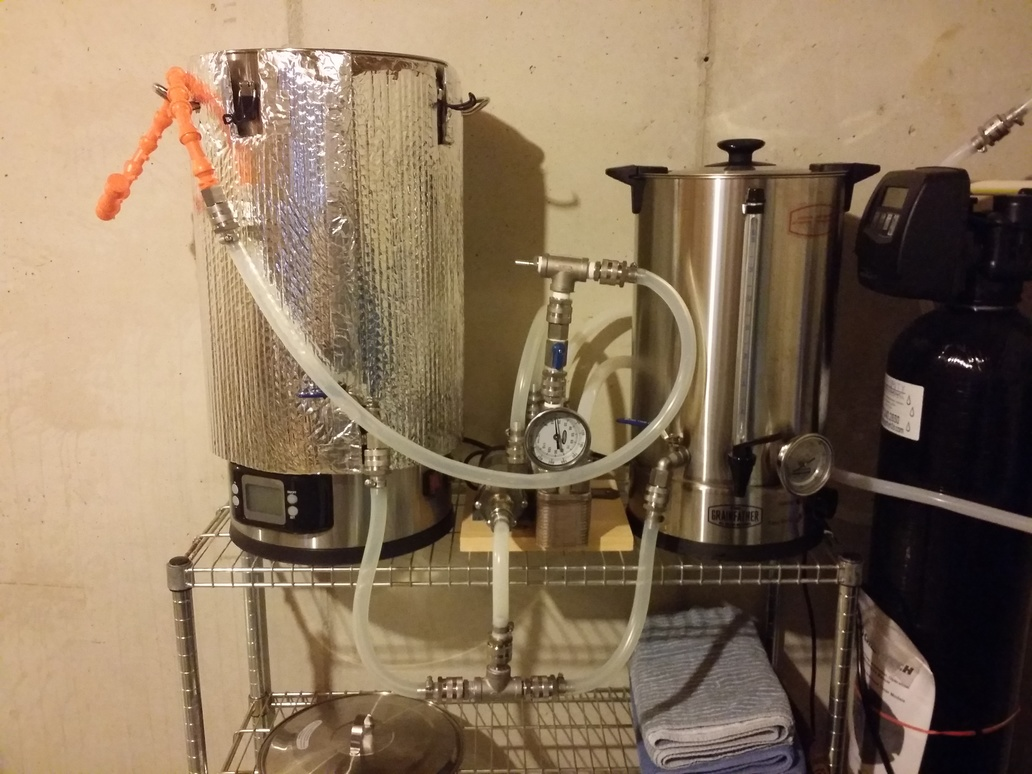
\includegraphics[width=\textwidth]{IMG_20190126_081006_reduced}
  \caption{Setting up for Brew}\label{fig:brew:setup}
\end{figure}

\begin{figure}[H]
  \centering
  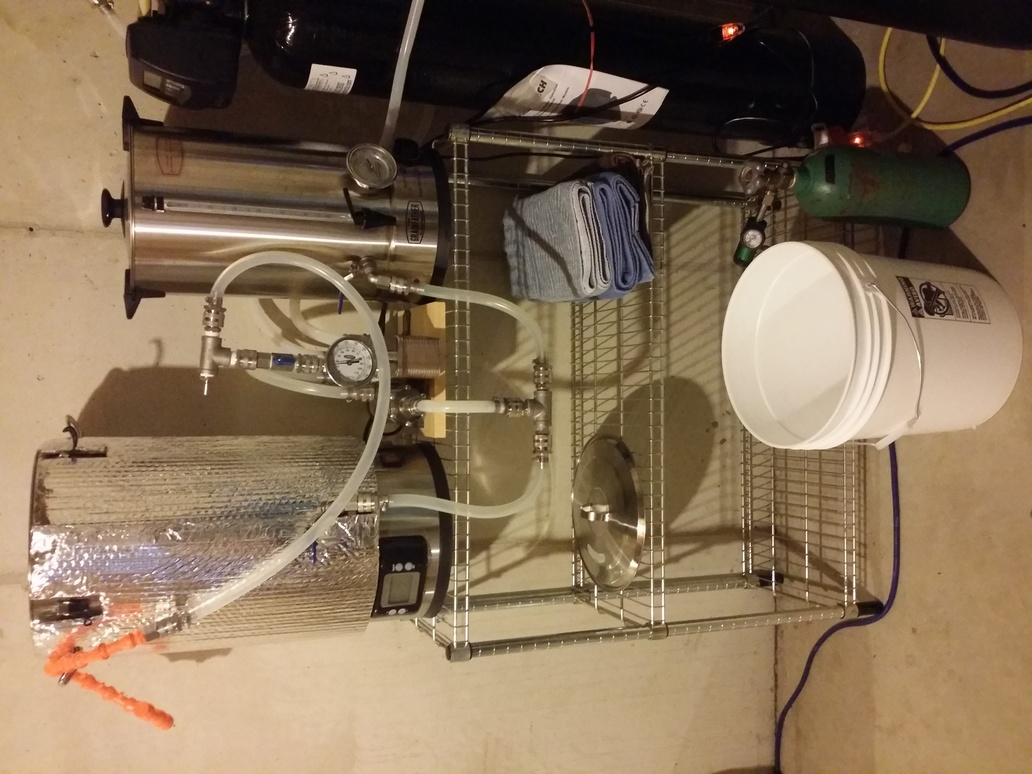
\includegraphics[angle=270,origin=c,width=0.5\textwidth]{IMG_20190126_081031_reduced}
  \caption{Setting up for Brew}\label{fig:brew:setup2}
\end{figure}

\begin{figure}[H]
  \centering
  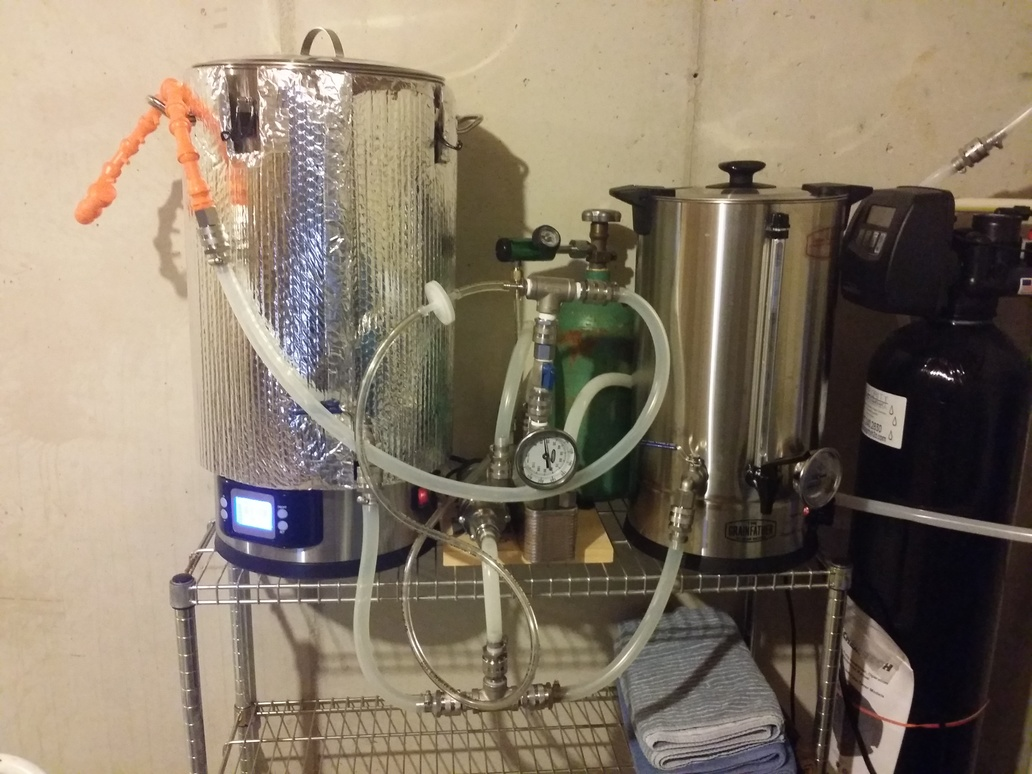
\includegraphics[width=\textwidth]{IMG_20190126_182020_reduced}
  \caption{Setting up for Brew}\label{fig:brew:setup3}
\end{figure}

\begin{figure}[H]
  \centering
  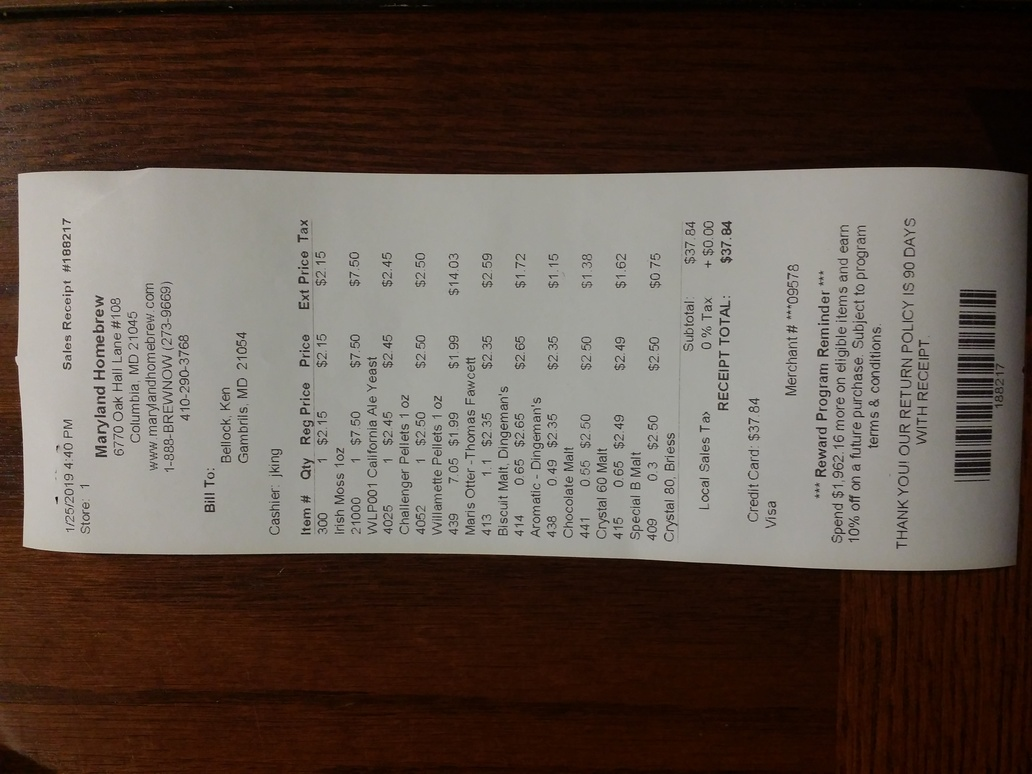
\includegraphics[angle=270,origin=c,width=0.5\textwidth]{IMG_20190126_190856_reduced}
  \caption{Brew Receipt}\label{fig:brew:receipt}
\end{figure}

\begin{figure}[H]
  \centering
  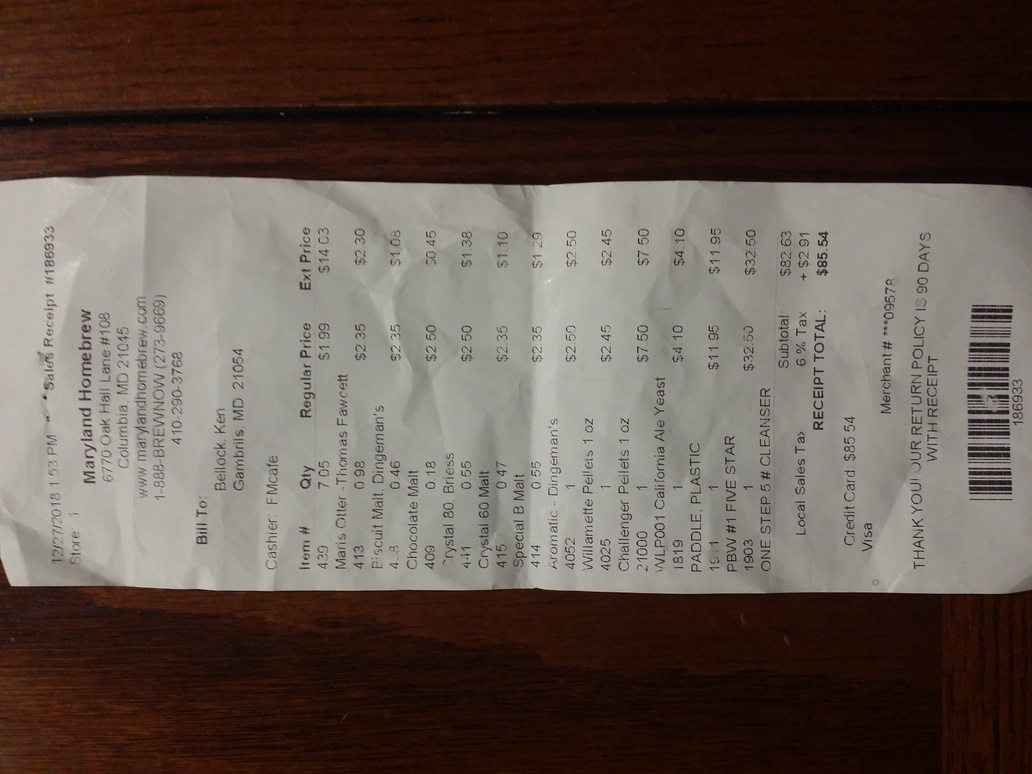
\includegraphics[angle=270,origin=c,width=0.5\textwidth]{IMG_20190126_191149_reduced}
  \caption{Brew Receipt}\label{fig:brew:receipt}
\end{figure}

\begin{figure}[H]
  \centering
  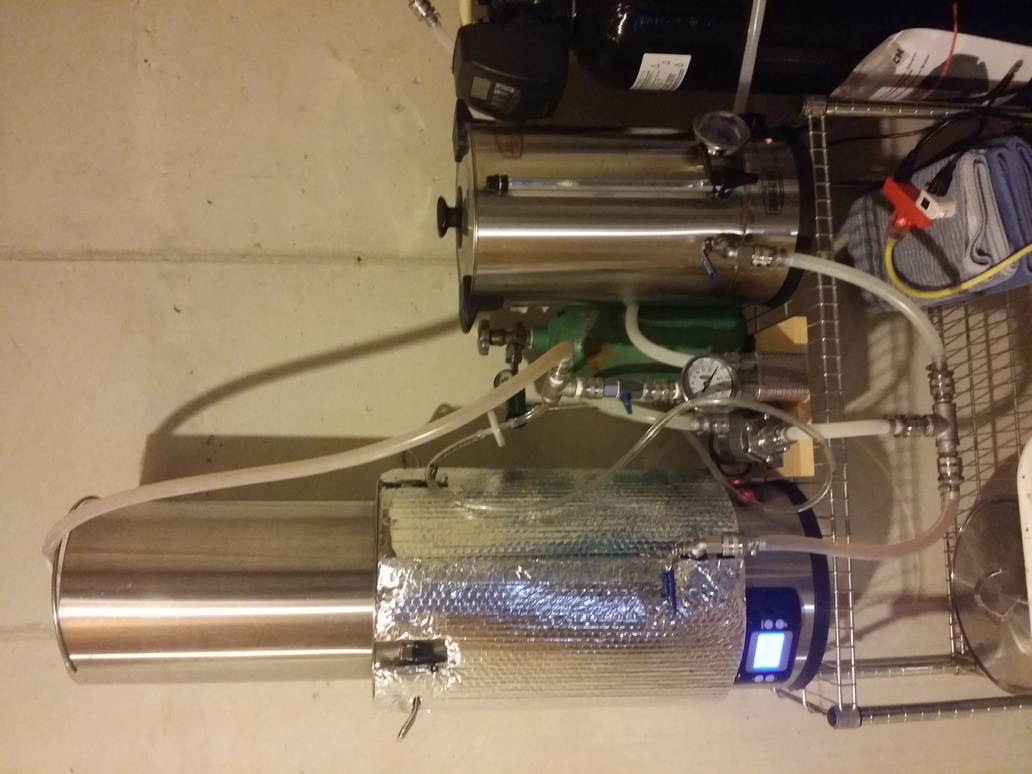
\includegraphics[angle=270,origin=c,width=0.5\textwidth]{IMG_20190126_195156_reduced}
  \caption{Sparging}\label{fig:brew:sparge}
\end{figure}

\begin{figure}[H]
  \centering
  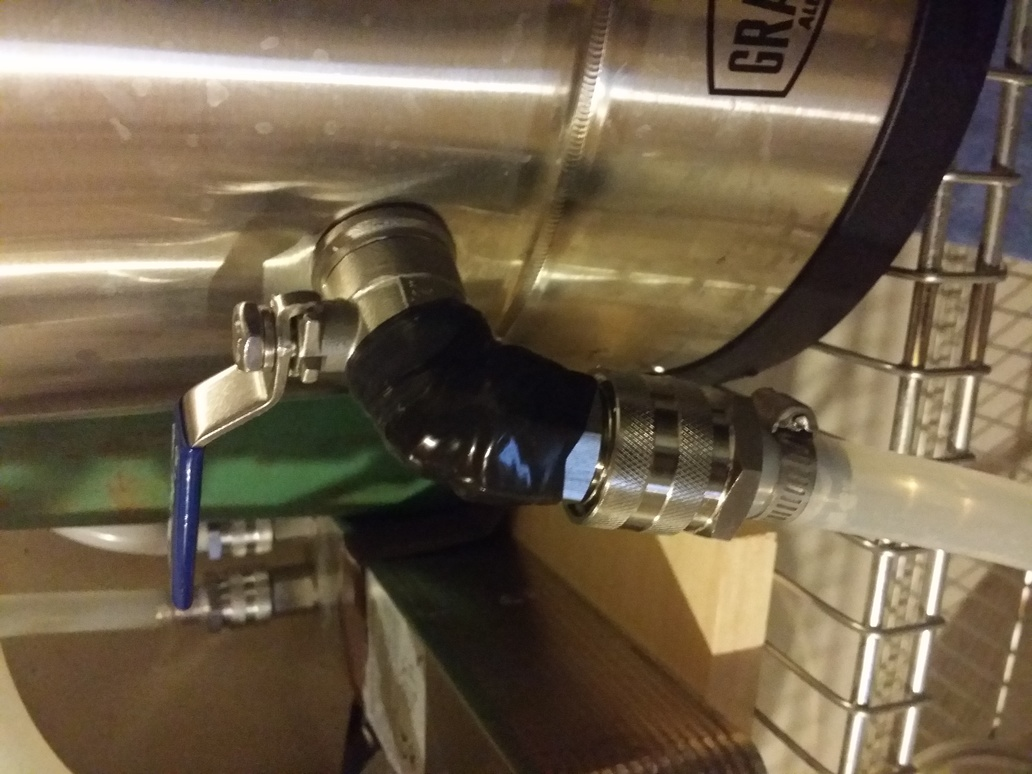
\includegraphics[angle=270,origin=c,width=0.5\textwidth]{IMG_20190126_203251_reduced}
  \caption{Patch for leak}\label{fig:brew:leak}
\end{figure}

\begin{figure}[H]
  \centering
  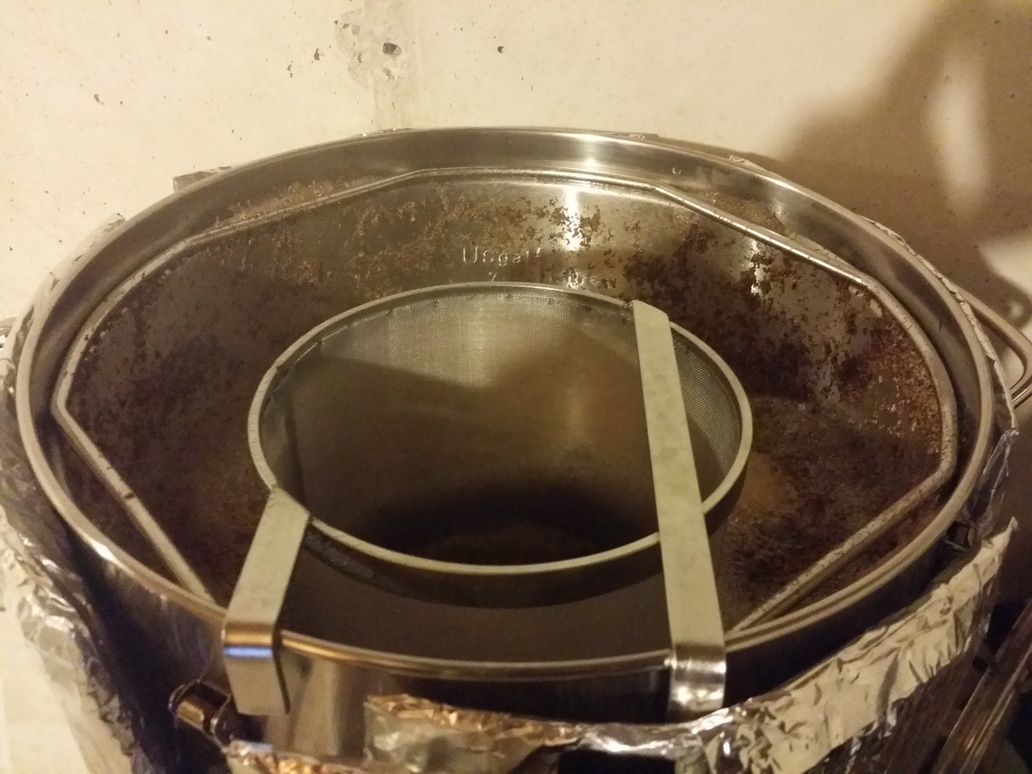
\includegraphics[width=\textwidth]{IMG_20190126_211535_reduced}
  \caption{Hop Additions}\label{fig:brew:hopadditions}
\end{figure}

\begin{figure}[H]
  \centering
  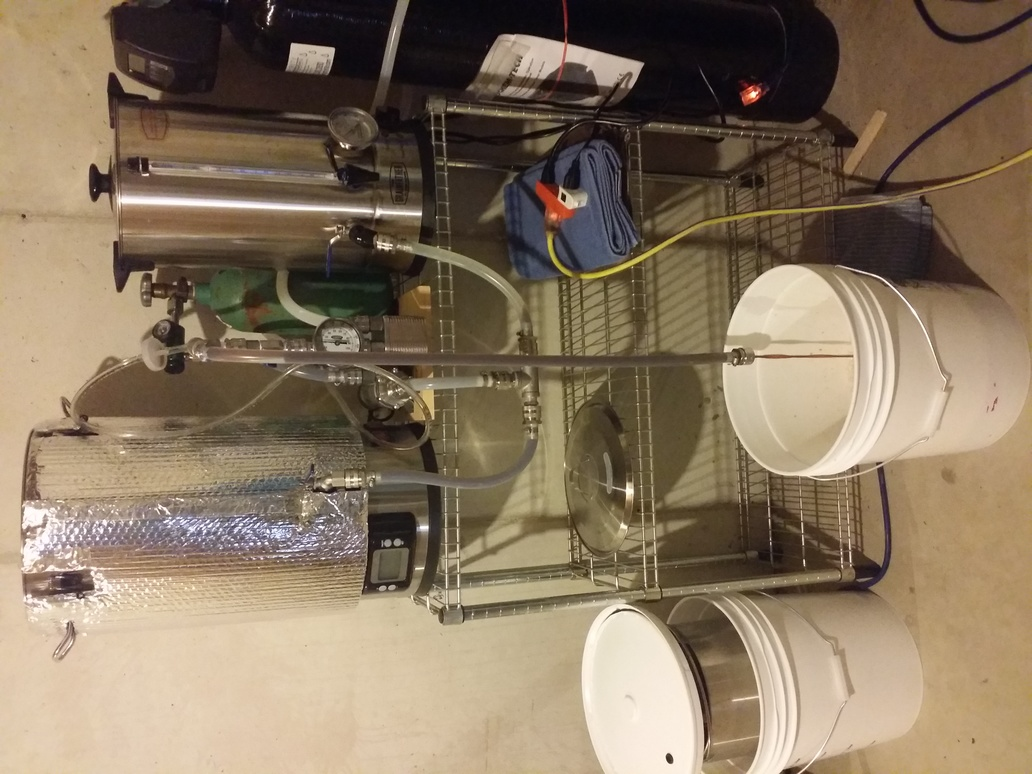
\includegraphics[angle=270,origin=c,width=0.5\textwidth]{IMG_20190126_222126_reduced}
  \caption{Chilling and transfer to Primary Fermentation}\label{fig:brew:chilling}
\end{figure}

\begin{figure}[H]
  \centering
  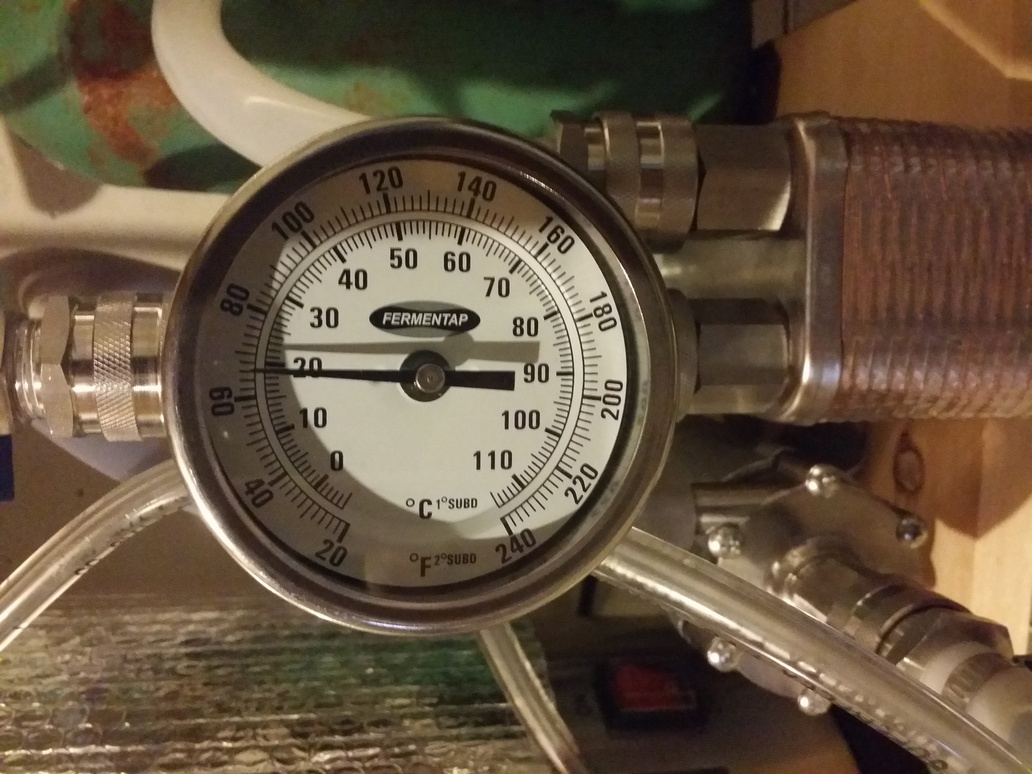
\includegraphics[angle=270,origin=c,width=0.5\textwidth]{IMG_20190126_222143_reduced}
  \caption{Temperature Exiting Plate Chiller}\label{fig:brew:chilltemp}
\end{figure}

\begin{figure}[H]
  \centering
  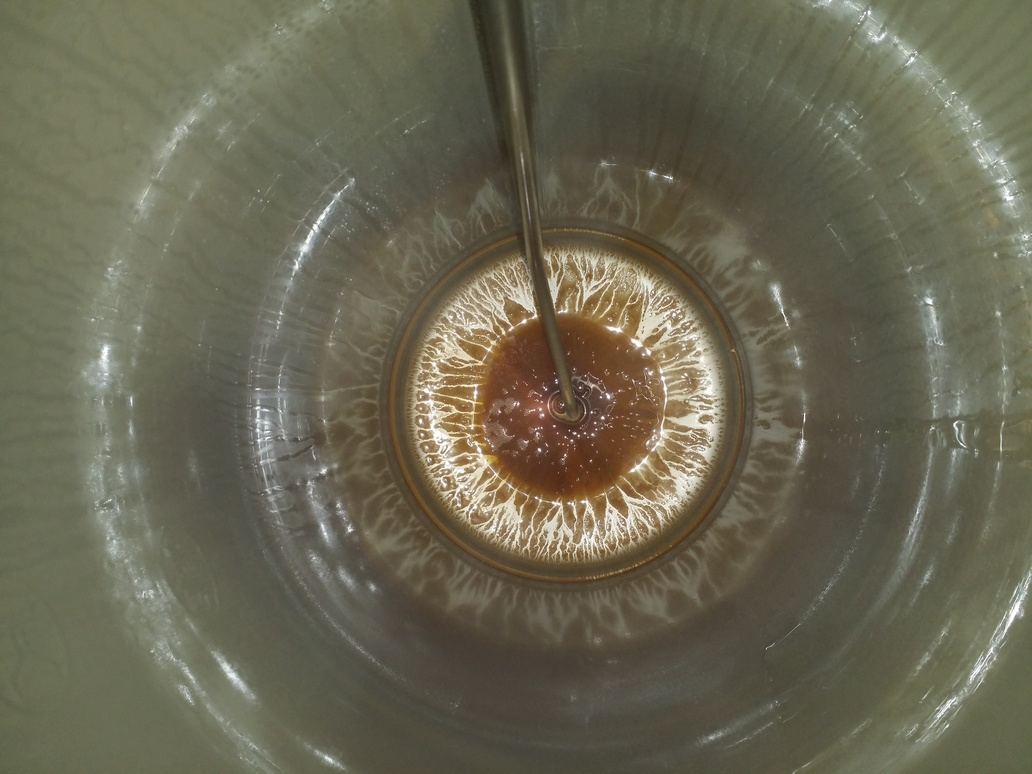
\includegraphics[width=\textwidth]{IMG_20190127_080524_reduced}
  \caption{Sediment at bottom of empty keg}\label{fig:keg1:empty}
\end{figure}

\begin{figure}[H]
  \centering
  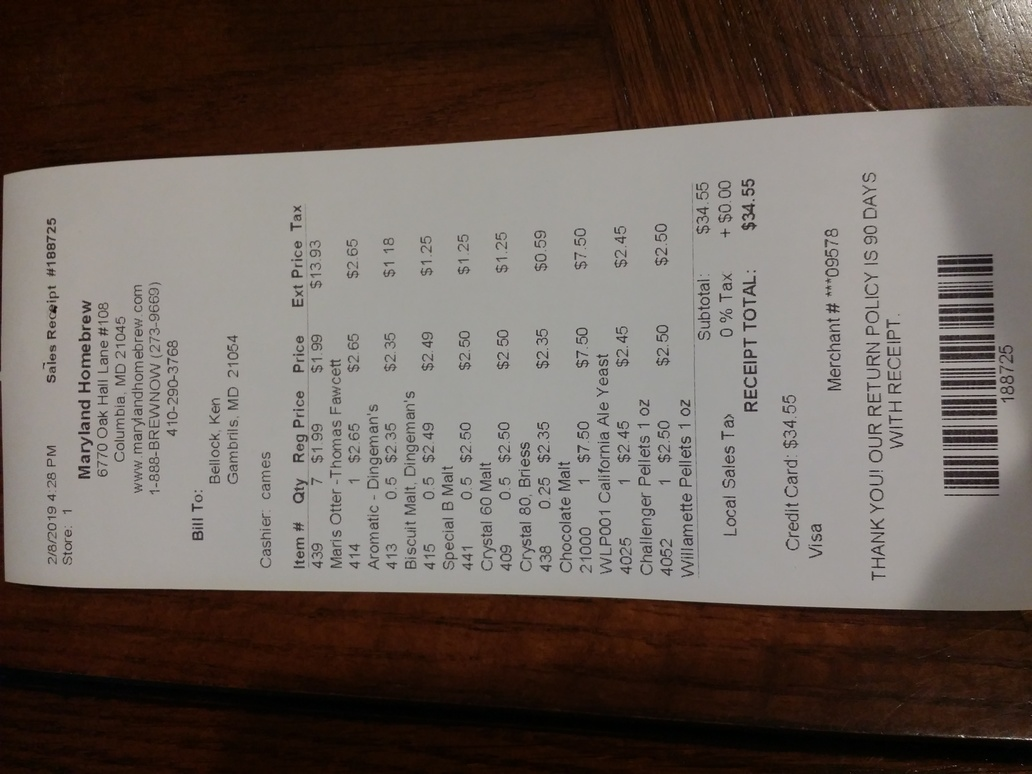
\includegraphics[angle=270,origin=c,width=0.5\textwidth]{IMG_20190208_185003_reduced}
  \caption{Receipt}\label{fig:brew:receipt}
\end{figure}

%------------------------------------------------------------------------------
\def\todaysdate{20190209}
\newday{\todaysdate}\label{\todaysdate}

\newentry[Brew]{0754 Brew}
\FloatBarrier{}
0754 Start Heating water.  Filled to 4.5 gallon mark on mash tun, set temperature to 163.  Put 13.5 liters in the sparge water heater, and started heat

0759 Mixed one gallon of one step cleaner/sanitizer

0845 Water is up to 163 in the mash tun. Reduced temperature setting of mash tun to 152, starting mash in

0855 Ended Mash In, temperature at 160.  Reduced temperature setting of mash tun to 152.  Note: I would have been closer to the 152 target if I had lowered the temperature setting before mash in.  I noticed when I was done mashing in the heater had been running the whole 10 minutes.  Leaving lid off to let temperature drop to target temp faster.

0938 Mash tun temp down to 152, placed lid back on

0955 Raised mash tube up, started pump at slow pace to recirculate wort

1025 Starged sparging, targeting 8L of water for sparging, turned on heater to start getting up to boil temperature

Note:  Sparging slow as I should, I am taking too long, for recirculating for 30 minutes.  Next time recirculate for only 10 minutes after raising the mash tube.

Note:  Sparge water in tank reads 168, exiting the plate chiller at 158, and going into the mash tube at 148

1118 8 Liters completed sparging, letting wort finish draining from grain bed.

Note: New strategy, recirculate 10 minutes, sparge 50-60, and end of sparge, turn on heater to 220, and let the mash tube sit on top until boil is reached.

1149 Removed grain bed, wort level is just below the 5.5 gal mark on the mash tun

1200 Boil started, added challenger hops in hop spider

1245 Added 1 teaspoon irish moss

\begin{figure}[H]
  \centering
  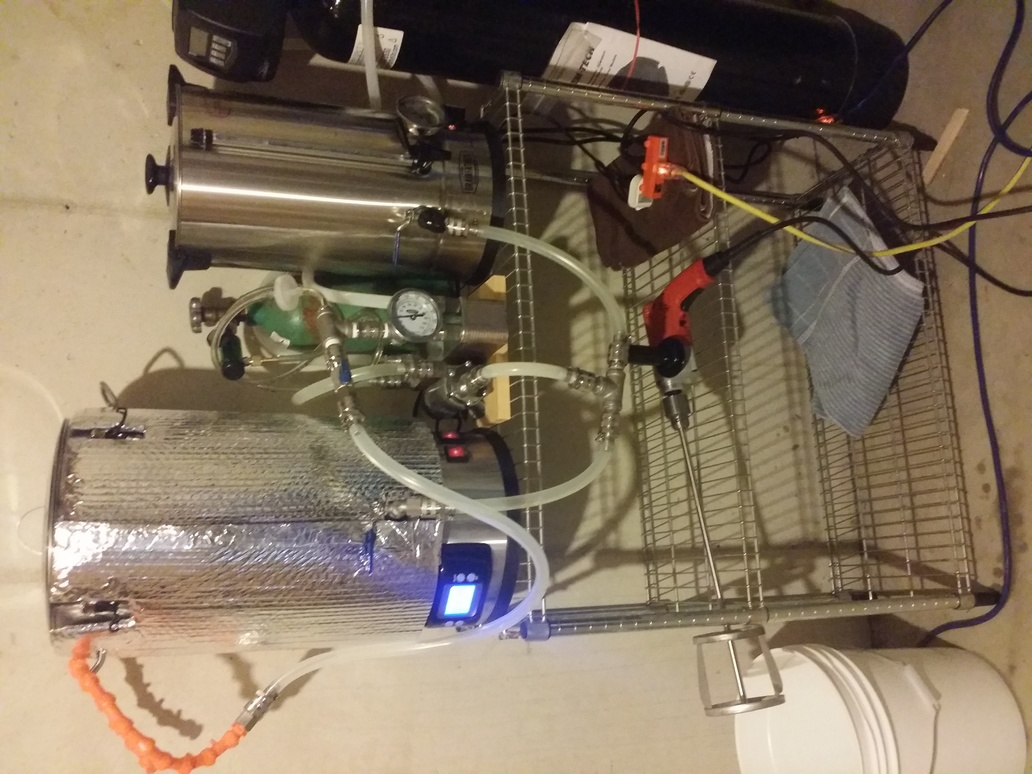
\includegraphics[angle=270,origin=c,width=0.5\textwidth]{IMG_20190209_082312_reduced}
  \caption{Setting up for brew}\label{fig:brew:setup}
\end{figure}

\begin{figure}[H]
  \centering
  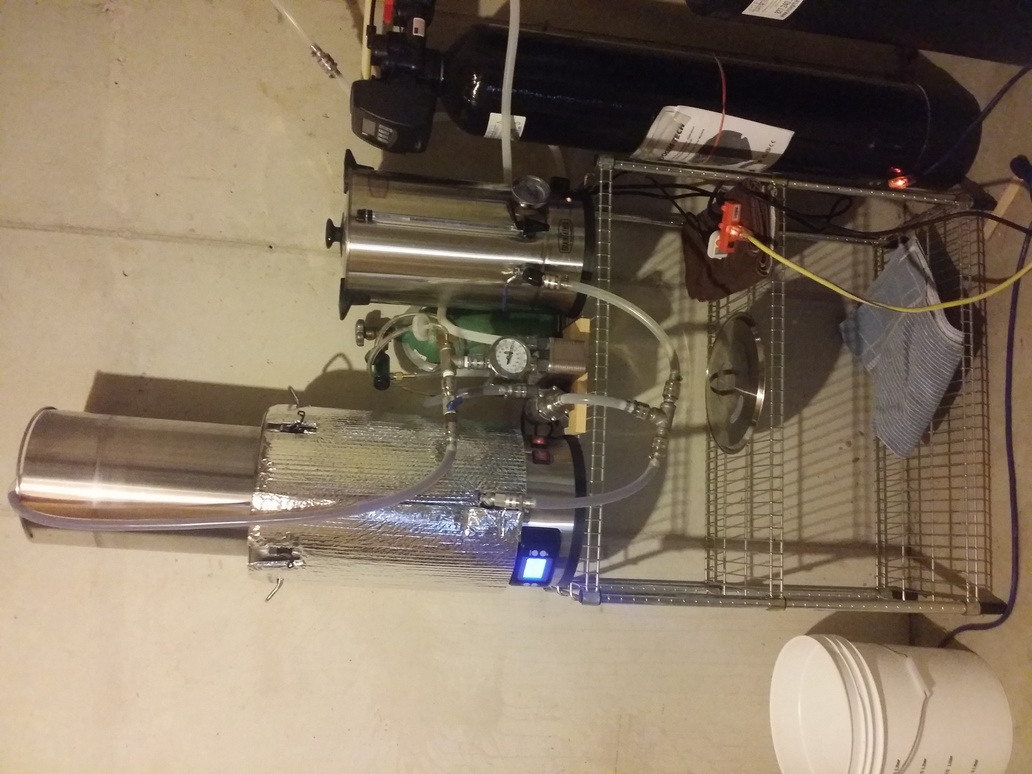
\includegraphics[angle=270,origin=c,width=0.5\textwidth]{IMG_20190209_101016_reduced}
  \caption{Sparging}\label{fig:brew:sparge}
\end{figure}

\begin{figure}[H]
  \centering
  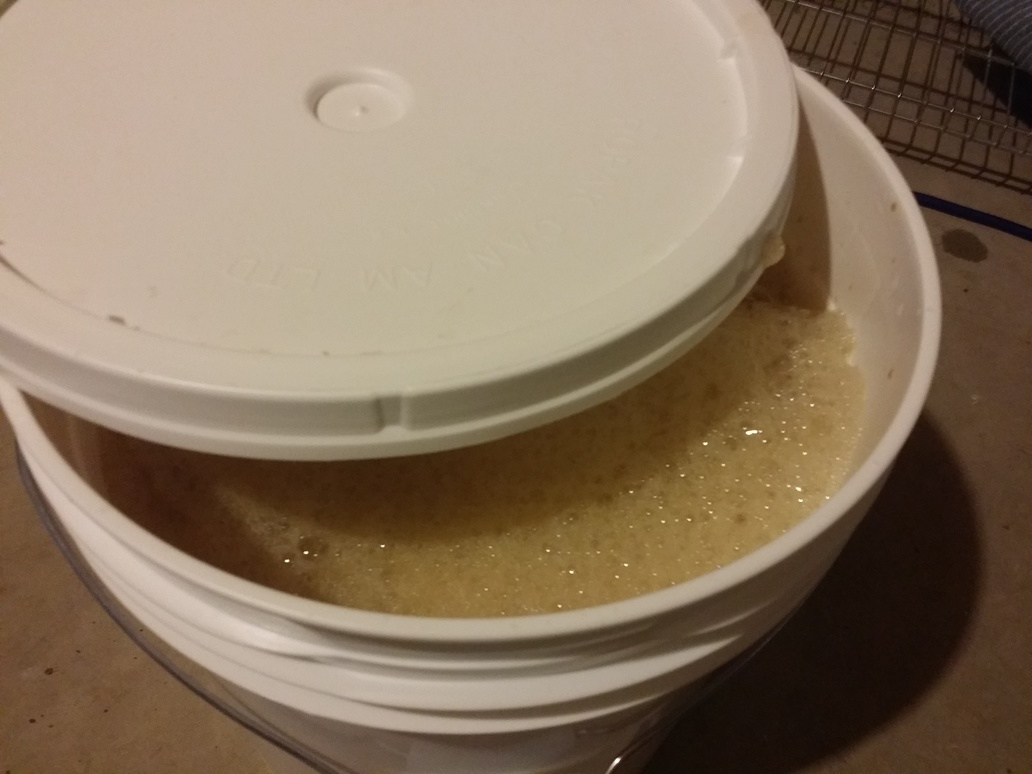
\includegraphics[width=\textwidth]{IMG_20190209_131702_reduced}
  \caption{Aeration Complete}\label{fig:brew:aeration}
\end{figure}

\begin{figure}[H]
  \centering
  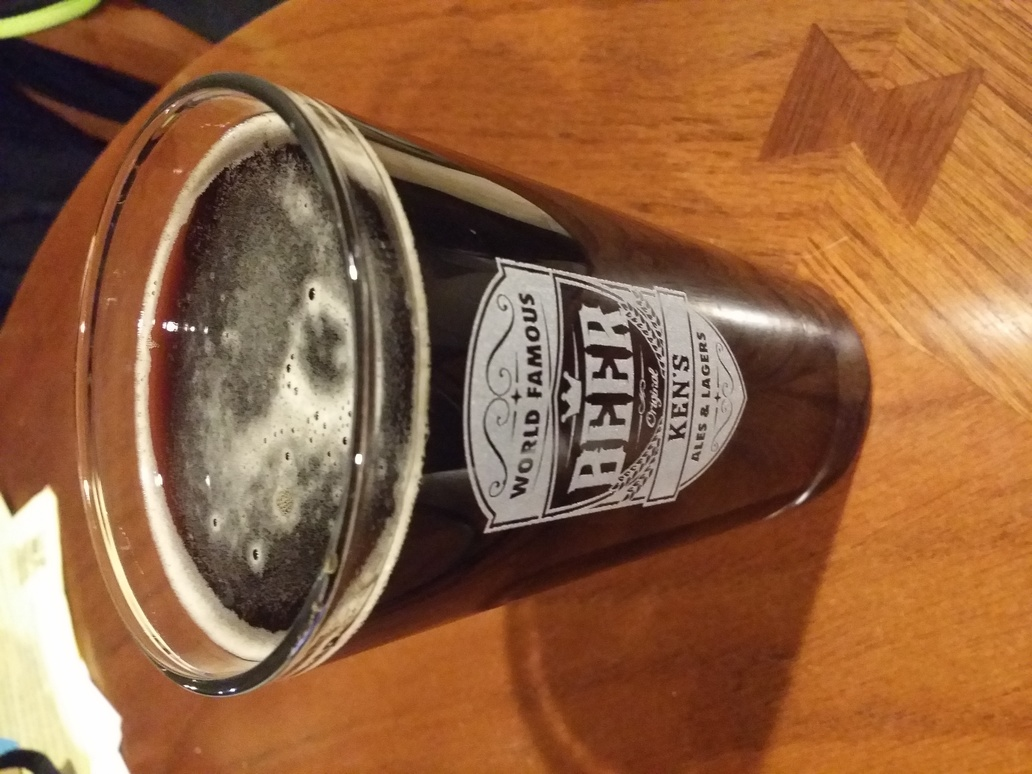
\includegraphics[angle=270,origin=c,width=0.5\textwidth]{IMG_20190213_212835_reduced}
  \caption{Sample Pour}\label{fig:sample:pour}
\end{figure}

\begin{figure}[H]
  \centering
  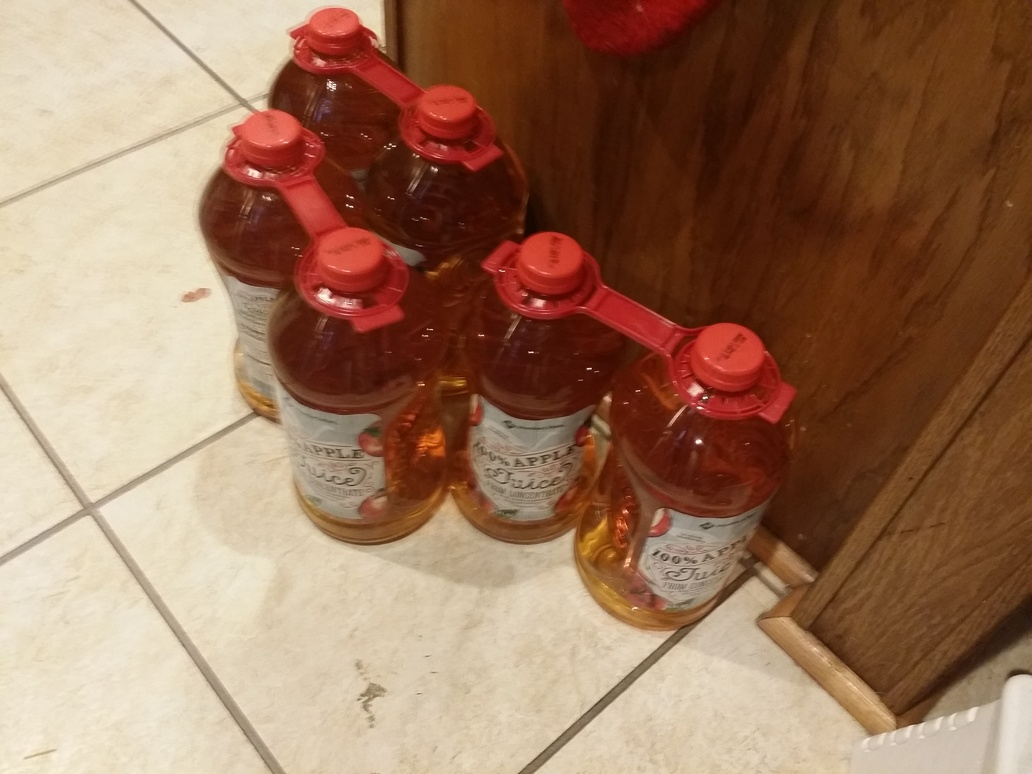
\includegraphics[width=\textwidth]{IMG_20190223_190343_reduced}
  \caption{Juice for Cider}\label{fig:brew:juice}
\end{figure}

\begin{figure}[H]
  \centering
  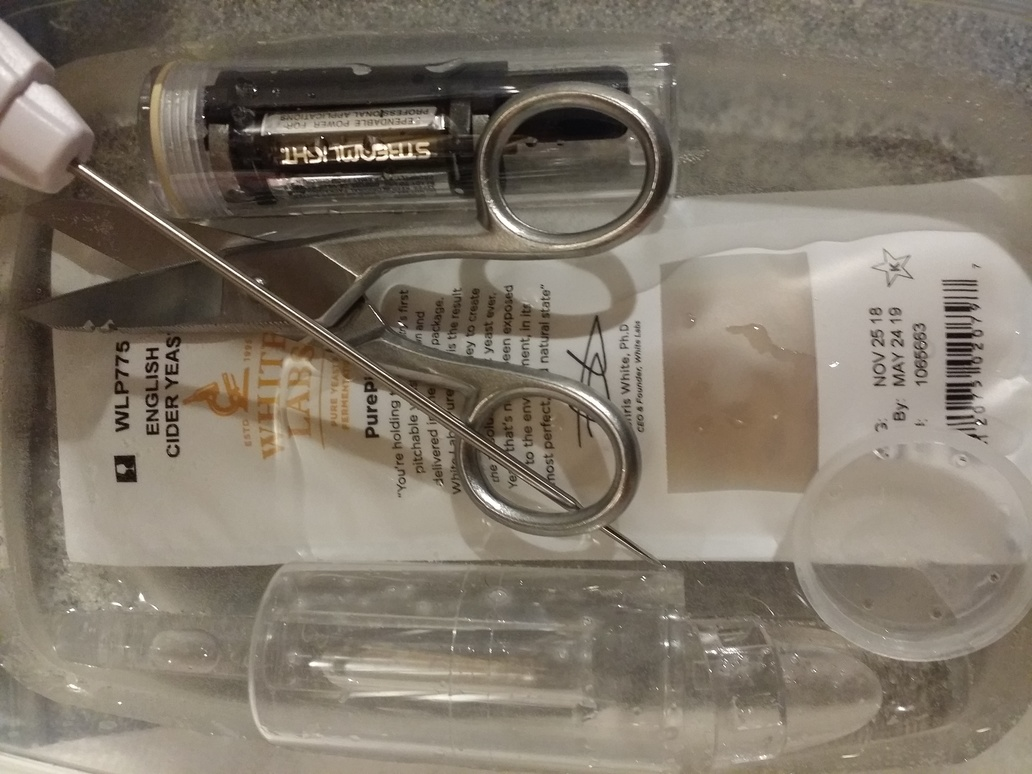
\includegraphics[width=\textwidth]{IMG_20190223_190405_reduced}
  \caption{Sanitizing for Cider}\label{fig:brew:sanitizing}
\end{figure}

\begin{figure}[H]
  \centering
  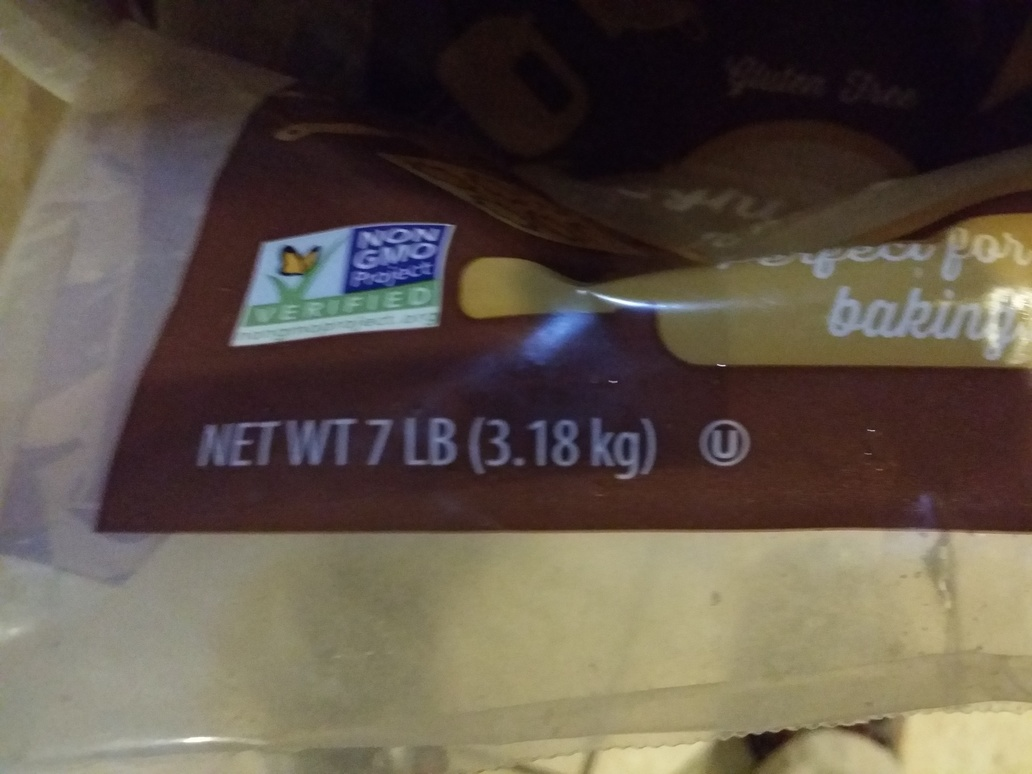
\includegraphics[width=\textwidth]{IMG_20190223_190424_reduced}
  \caption{Brown Sugar for Cider}\label{fig:brew:brownsugar}
\end{figure}

\begin{figure}[H]
  \centering
  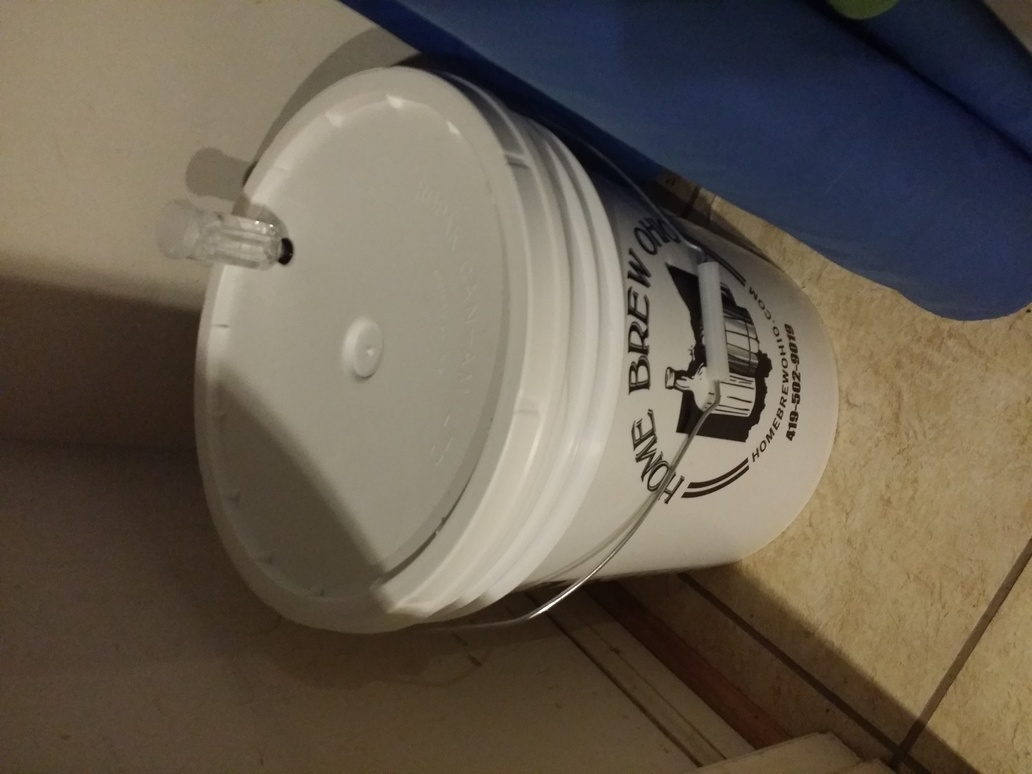
\includegraphics[angle=270,origin=c,width=0.5\textwidth]{IMG_20190223_194644_reduced}
  \caption{Beginnign of Primary Fermentation}\label{fig:brew:primary}
\end{figure}

\begin{figure}[H]
  \centering
  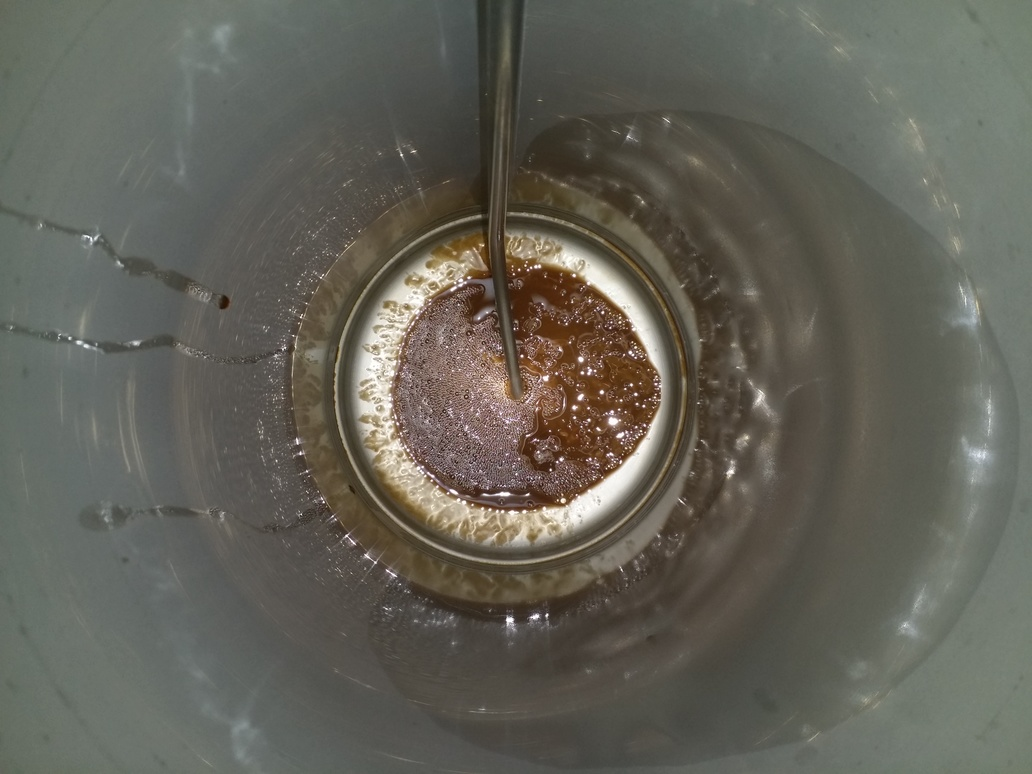
\includegraphics[width=\textwidth]{IMG_20190225_171122_reduced}
  \caption{Sediment at Empty Keg}\label{fig:keg2:empty}
\end{figure}

\begin{figure}[H]
  \centering
  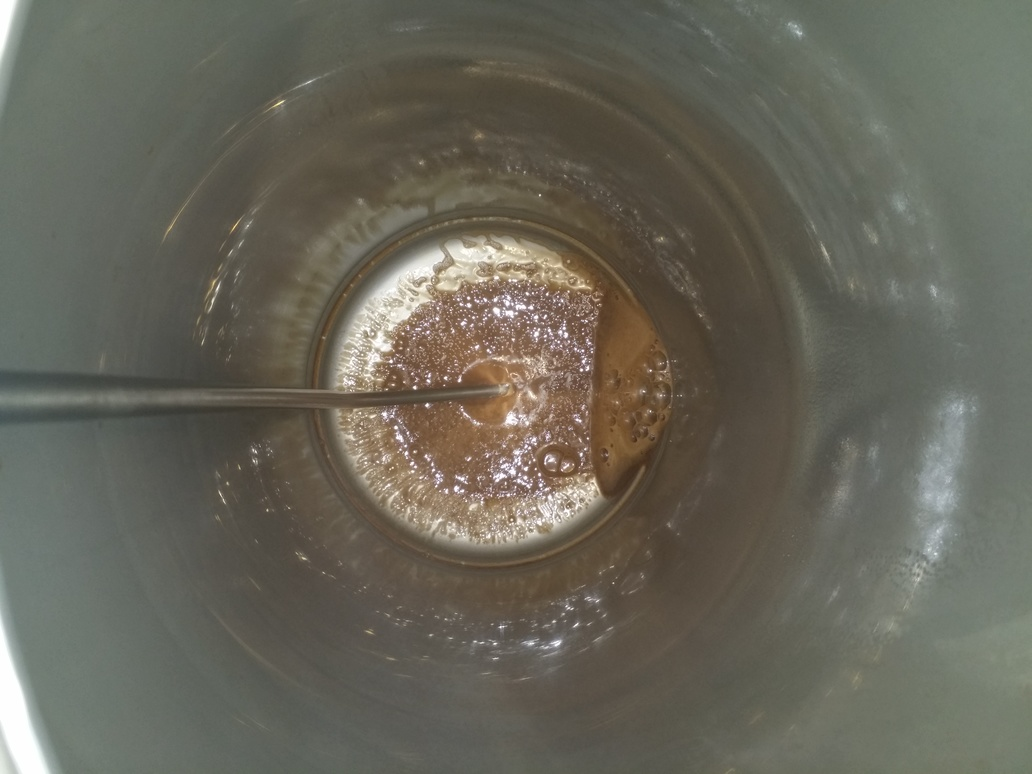
\includegraphics[width=\textwidth]{IMG_20190305_090133_reduced}
  \caption{Sediment at Empty Keg}\label{fig:keg3:empty}
\end{figure}

\begin{figure}[H]
  \centering
  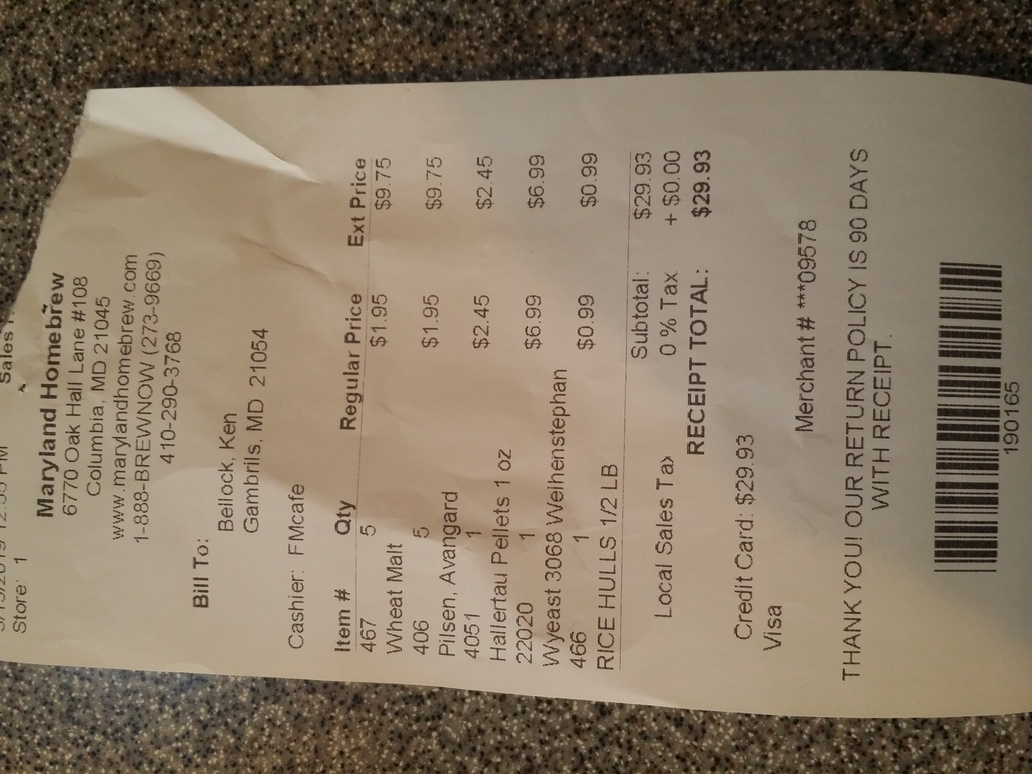
\includegraphics[angle=270,origin=c,width=0.5\textwidth]{IMG_20190315_181311_reduced}
  \caption{Receipt}\label{fig:brew:receipt}
\end{figure}

%------------------------------------------------------------------------------
\def\todaysdate{20190317}
\newday{\todaysdate}\label{\todaysdate}

\newentry[Brew]{0700 Brew}
0700 Placed 4 gallons in mash tun and set heater to 130, 5 gallons in sparge water heater
0728 Set mash tun temperature to 120 and began mash in
0834 Mash in complete, beginning 20 minute protein rest, mash temp at 119
0835 Set mash tun temperature to 110 as re-inspection of the recipie listed 110
0854 Increased temperature to 152 and began slow recirculation
0916 152 degrees in mash tun, starting 1 hour mash with slow recirculation continuing
1016 Raised grain tube, set the heater to 168, and continued reciculating for 10 minutes.
1026 Closed valve on the mash tun and opened the valve on the sparge water heater.  Targeting 11L of sparge water.
1044 13L of sparge water transferred, turned off pump and closed the valve on the sparge water.  Set the mash tun temperature to 220.
1112 Collected enough wort to fill up to the 5.5 gallon mark on the mash tun.  Removed the mash tube, and placed empty hop spider into the wort to break the surface tension at boil.
1114 Boil started, began 30 minute timer for hop addition
1145 Added hops to hop spider
1240 Started Recirculating water to sanitize the pump and hose
1245 Turned off heat to the mash tun, tuned on water flow to the plate chiller, slowed flow till water temperature reading exiting the plate chiller was mid to low 60's, then turned on the oxygen and started transfer to the primary fermentation bucket.
1529 Done cleaning.

Note: Sparge heater set to 80 for sparging, set to 65 for warming cleaning water.
Note: Next time, remember to spray sanitizer in the oxygen fittings and stone, if there is an infection during fermentation, this is the vector.

%------------------------------------------------------------------------------
\def\todaysdate{20190324}
\newday{\todaysdate}\label{\todaysdate}

\newentry[Brew]{0730 Brew}
0730 Placed 4.5 gallons in mash tun and set heater to 162.  Connected all hoses, bags, and mixed one gallon of sanitizer.  Yeast packet was placed in tupperware with sanitizer along with the airtrap and the scissors.
0820 Set the mash tun temperature to 154 and began mash in
0830 Mash in complete, circulationi started, at the end of mash in temp is 159.
Note:  The check valve and cutoff for the oxygen was placed in the sanitizer solution, but a reaction occurred with the metal in the valve shutoff handle.  Everything in the sanitization solution was cleaned off, and a new sanitizer bath was poured and the check valve was sanitized again, but this time with alcohol.
0930 Raised temperature setting to 168
0940 Raised mash tube, continued recirculating wort
0950 Closed valve on the mash tun and opened the valve on the sparge water heater.  Targeting 11L of sparge water.
1127 11L of sparge water transferred, turned off pump and closed the valve on the sparge water.  Set the mash tun temperature to 220.
1200 Boil started, began 30 minute timer for hop addition
1230 Added hops to hop spider
1325 Started Recirculating water to sanitize the pump and hose
 Turned off heat to the mash tun, tuned on water flow to the plate chiller, slowed flow till water temperature reading exiting the plate chiller was mid to low 60's, then turned on the oxygen and started transfer to the primary fermentation bucket.
 Done cleaning.

%------------------------------------------------------------------------------
\def\todaysdate{20190511}
\newday{\todaysdate}\label{\todaysdate}

\newentry[Brew]{0710 Brew}
Startup Notes.
\begin{my_itemize}
  \item The mash tun was filled with exactly 4 measured gallons of water.  The water line in the mash tun came up half a gallon below the 4 gallon mark.  One half gallon was added, and the water level was exactly at 4 gallons.  The water was drained out, and the dead space at the bottom of the mash tun below the valve was just a little less than half a gallon.  Their lines must not account for the dead space.  To start with 4.5 gallons of water, water needs to be filled to the 4 gallon mark in the mash tun.
  \item The chapman stainless steel fermentation buckets are about a quarter gallon off.  Two gallons of water reads about 1.75 on the gradations on the bucket.
\end{my_itemize}
0710 Start 4.5 Gallon in mash tun at 160
0750 Reached Temp
0810 Set mash tun to 154 deg, started Mash In
0820 Mash in complete temp at 148
0920 Raised temperature setting to 168
0930 Raised mash tube, Closed valve on the mash tun and opened the valve on the sparge water heater.  Targeting 11L of sparge water.
1026 10L of sparge water transferred, turned off pump and closed the valve on the sparge water.  Set the mash tun temperature to 220.
1100 While heating up to boiling, another 5L of water was added to adjust the gravity the refractometer read 1.048 
1110 Boil Started
1250 Begin Transfer

1330 Start 4.5 Gallon in mash tun at 161
1400 Reached Temp
1415 Set mash tun to 154 deg, started Mash In
1420 Mash in complete temp at 154
1520 Raised temperature setting to 168
1530 Raised mash tube, Closed valve on the mash tun and opened the valve on the sparge water heater.  Targeting 11L of sparge water.
1620 11L of sparge water transferred, turned off pump and closed the valve on the sparge water.  Set the mash tun temperature to 220.
1647 Boil Started SG 1.041
0710 Finished Cleaning

%------------------------------------------------------------------------------
\def\todaysdate{20190706}
\newday{\todaysdate}\label{\todaysdate}

\newentry[Brew]{0710 Brew}

Original Recipe

\begin{verbatim}
Schneider Weisse Aventinus tap 6 clone

5000g wheat malt
2000g Munich malt EBC 20
1000 Caramunch malt EBC 50
2000g Pilsner malt

Stepped mash:
30 minutes@50C in 15litres
Protein rest with grist/ liquor ratio 1:1.15
Raise to 65c for 60 mins with 8litres @ 100c
Sparge @72C to collect 25 litres wort.

Boil:
40g Hallertau Herbrucker@70 mins
10 g H H @ 15 mins
5g Irish Moss @15

Collected 18 litres.
Wyeast 3068 Weihenstephan Weizen
OG 1058
FG 1016
\end{verbatim}

\begin{description}
    \item[5000g] Wheat Malt
    \item[2000g] Munich Malt
    \item[2000g] Pilsner Malt
    \item[1000g] Caramunich Malt
\end{description}

Stepped Mash
\begin{enumerate}
  \item 30 Minutes at 120$^{\circ}$F in 4 gallons of liquor.
  \item Raise to 150$^{\circ}$ for 60 Minutes
  \item Sparge
\end{enumerate}

Boil
\begin{enumerate}
    \item Boil 90 Minutes
    \item 40g Hallertau Hersbrucker (4\% alpha acids): -70 Minutes
    \item 10g Hallertau Hersbrucker (4\% alpha acids): -15 Minutes
    \item 5g Irish Moss: -15 Minutes
\end{enumerate}

Target OG: 1.058
Target FG: 1.016

%------------------------------------------------------------------------------
\def\todaysdate{20190707}
\newday{\todaysdate}\label{\todaysdate}

\newentry[Brew]{1100 Brew}
Brewing Cider

\begin{itemize}
    \item Boiled .75 gallons of applejuice with 7 lbs of light brown sugar.
    \item Sanitized lids of applejuice, fermentation bucket, air trap, tilt sensor, and scissors.
    \item While bringing brown sugar and apple juice to a boil, the fermentation bucket was filled with the remainder of apple juice and the blender attachment was run to oxygenate the juice.
    \item The brown sugar and juice mixture was boiled for 5 minutes, then poured into the fermentation bucket.
    \item The resulting temperature in the fermentation bucket was 75 degrees, which was safe for the yeast, so the yeast was pitched, and then the blender was used for 10 minutes to continue oxygenating the mixture.
    \item The tilt sensor was added to the bucket, and the lid was secured and air lock filled with sanitizer.
    \item The fermentation bucket was placed in the kegerator at 68 degrees.
\end{itemize}

%------------------------------------------------------------------------------
\def\todaysdate{20190710}
\newday{\todaysdate}\label{\todaysdate}

\newentry[Inventory]{1700 Loading Inventory}
\FloatBarrier{}
1. Munich Malt Lite
2. Pilsen Malt
3. Caramunich (5/29/19)
4. Wheat Malt

\newentry[Brew]{1730 Brew}
\FloatBarrier{}
1730 Start Heating water.  Filled to 4.0 gallon mark on mash tun, which equates to 4.5 gallons of water, set temperature to 160.  Put 13.5 liters in the sparge water heater, and started heat

1815 Water is up to 162 in the mash tun. Reduced temperature setting of mash tun to 152, starting mash in

1820 Ended Mash In, temperature at 151.  Starting recirculation.

1920 Raised mash tube up. Starged sparging, targeting 7.5L of water for sparging over approximately an hour.  Setting temperature of kettle to 170.

2018 7.5 Liters completed sparging, letting wort finish draining from grain bed.  Set the kettle temperature to 220 to bring the wort to a boil.

2049 Removed grain bed, wort level is just below the 5.5 gal mark on the mash tun

2053 Boil started, added challenger hops 1oz 7.8\% in hop spider.  Collected just under the 5 gallon mark on kettle, which is 5.45 gallons or so.  Gravity at Boil is: 1.048

2138 Added 1 teaspoon irish moss

2148 Added 1oz Willamette 4.2\%

2153 Boil Complete.  Trasfer to primary fermentation bucket with yeast at 66 degrees.

Target OG: 1.050
Target Temperature: 66F

%------------------------------------------------------------------------------
\def\todaysdate{20190807}
\newday{\todaysdate}\label{\todaysdate}

\newentry[Brew]{1630 Brew}
\FloatBarrier{}
1630 Start Heating water.  Filled to 4.0 gallon mark on mash tun, which equates to 4.5 gallons of water, set temperature to 160.  Put 15.2 liters in the sparge water heater, and started heat

1720 Water is up to 162 in the mash tun. Reduced temperature setting of mash tun to 152, starting mash in

1726 Ended Mash In, temperature at 151.  Starting recirculation.

1826 Raised mash tube up. Starged sparging, targeting 7.0L of water for sparging over approximately an hour.  Setting temperature of kettle to 170.

1855 7.0 Liters completed sparging, letting wort finish draining from grain bed for remaining hour.

1926 Set the kettle temperature to 220 to bring the wort to a boil.

1950 Removed grain bed at 210 degrees, wort level is just below the 5.5 gal mark on the mash tun

1952 Boil started, since the boil is not as rigorous as I would like, we will add 15 minutes of boil before starting the one hour timer.

2007 Added challenger hops 1oz 7.8\% in hop spider.  Collected just under the 5 gallon mark on kettle, which is 5.4 gallons or so.  Gravity at Boil is: 1.051

2052 Added 1 teaspoon irish moss

2102 Added 1oz Willamette 4.2\%.  Started circulating through the plate chiller to sanitize everything for remaining 5 minutes.  Heat is on full.

2107 Boil Complete.  Trasfer to primary fermentation bucket with yeast at 66 degrees.

Actual OG: 1.056
Actual Temperature: 71 degrees

Target OG: 1.050
Target Temperature: 66F

%------------------------------------------------------------------------------
\def\todaysdate{20191201}
\newday{\todaysdate}\label{\todaysdate}

\newentry[Brew]{0738 Brew}
\FloatBarrier{}
0738 Start Heating water.  Filled to 4.0 gallon mark on mash tun, which equates to 4.5 gallons of water, set temperature to 130.  Put 15.2 liters in the sparge water heater, and started heat

1108 Water is up to 130 in the mash tun. Reduced temperature setting of mash tun to 120, starting mash in

1119 Ended Mash In, temperature at 120.  Starting recirculation.

1149 Raised temperate in mash tube to 150.  When the heater kicked in a air sucking noise could be heard, and then error E4 was displayed on the screen stating dry.  I added two liters of water from the sparge water tank, and slowed the pump rate down.  The sparge water is at 170, so it will help to raise the temperature up.  I'm hoping the additional water will be enough to resuming heating through the mash tun.  After several tries to get E4 to go away, I added a bunch of water down the inside of the mash tube in an attempt to was off the sensor.  The water inside this space filled to one inch from the top while doing this.  I still got E4.  I read online there is a reset switch underneath the unit.  I pressed this switch, and the heater is now working.  

1223 We have reached 150, restarting one hour timer from here.

1323 Raised mash tube up. Starged sparging, targeting 10.0L of water for sparging over approximately an hour.  Setting temperature of kettle to 170.

1500 10.0 Liters completed sparging, letting wort finish draining from grain bed for remaining hour.

1500 Set the kettle temperature to 220 to bring the wort to a boil.

1600 Removed grain bed at 210 degrees, wort level is just below the 5.5 gal mark on the mash tun

1600 Boil started, since the boil is not as rigorous as I would like, we will add 15 minutes of boil before starting the one hour timer.

1625 Added challenger hops 1oz 7.8\% in hop spider.  Collected just under the 5 gallon mark on kettle, which is 5.4 gallons or so.  Gravity at Boil is: 1.051

1720 Added 1 teaspoon irish moss and .5 oz hops

1730 Started circulating through the plate chiller to sanitize everything for remaining 5 minutes.  Heat is on full.

Boil Complete.  Trasfer to primary fermentation bucket with yeast at 66 degrees.

Actual OG: 
Actual Temperature: 

Target OG: 1.050
Target Temperature: 66F

%------------------------------------------------------------------------------
\def\todaysdate{20191229}
\newday{\todaysdate}\label{\todaysdate}

\newentry[Brew]{0749 Brew}
\FloatBarrier{}
0749 Start Heating water.  Filled to 4.5 gallon mark on mash tun, which equates to 5.0 gallons of water, set temperature to 130.  Put 16.0 liters in the sparge water heater, and started heat.  To make sure the lines did not take away from the volume, I circulated the pump to fill the lines.  When I did this a lot of black film like substance came out of the plate chiller.  In the future I will need to rince out the plate chiller before recirculating, and the idea also came up to switch sides on the plate chiller for running wort through such that every other brew the plate chiller will be thoroughly rinsed out with clean water from the well water side during cooling.

1055 Water is up to 130 in the mash tun. Reduced temperature setting of mash tun to 120, starting mash in.  For today's brew, I will not be using the bag, and will be hand mixing in the mash.  The goal here is to not allow so much flour and flakes to go through the false bottom and collect on the burner.  Hopefully this will reduce the occurance of the E4 error code I think is being caused by scalding of loose material on the burner.

1100 Ended Mash In, temperature at 120.  Starting recirculation.

1130 Raised temperate in mash tube to 150.  

1145 We have reached 150, restarting one hour timer from here.

1245 Raised mash tube up. Starged sparging, targeting 8.0L of water for sparging over approximately an hour.  Setting temperature of kettle to 185.

1320 8.0 Liters completed sparging, letting wort finish draining from grain bed for remaining hour.

1345 Set the kettle temperature to 220 to bring the wort to a boil.

1607 Removed grain bed at 210 degrees, wort level is at the 4.25 gal mark on the mash tun

1620 Boil started.

1625 Added challenger hops 1oz 7.8\% in hop spider.  Collected just under the 5 gallon mark on kettle, which is 5.4 gallons or so.  Gravity at Boil is: 1.051

1720 Added 1 teaspoon irish moss and .5 oz hops

1730 Started circulating through the plate chiller to sanitize everything for remaining 5 minutes.  Heat is on full.

Boil Complete.  Trasfer to primary fermentation bucket with yeast at 64 degrees.

Actual OG: 1.059
Actual Temperature: 64

Target OG: 1.050
Target Temperature: 66F
